\documentclass[11pt]{article}
% Shared preamble of the v4 papers (English; pdflatex).
\usepackage[T1]{fontenc}
\usepackage[utf8]{inputenc}
\usepackage{newtxtext,newtxmath}
\usepackage[margin=1in]{geometry}
\usepackage{microtype}
\usepackage{amsmath,amssymb}
\usepackage{booktabs,multirow,array}
\usepackage{graphicx}
\usepackage[font=small,labelfont=bf]{caption}
\usepackage{subcaption}
\usepackage{xcolor}
\usepackage{enumitem}
\usepackage[numbers,sort&compress]{natbib}
\usepackage[hidelinks]{hyperref}
\usepackage{url}
\setlist{nosep,leftmargin=*}
\newcommand{\kev}{Kev-4B}
\newcommand{\pc}{P_{\mathrm{c}}}
\newcommand{\pg}{P_{\mathrm{g}}}
\newcommand{\ci}[2]{[#1,\,#2]}
\newenvironment{correction}{\begin{center}\begin{minipage}{0.95\linewidth}\small\setlength{\parskip}{3pt}\noindent\textbf{Correction notice.}~}{\end{minipage}\end{center}}

% \NUM{key}: a number computed by dcjev/analysis/paper_numbers.py and written to the paper's numbers.tex.
% A key that numbers.tex does not define prints as ??key?? and logs a warning, so a missing number cannot vanish.
\makeatletter
\newcommand{\NUM}[1]{\ifcsname num@#1\endcsname\csname num@#1\endcsname\else\textbf{??\detokenize{#1}??}\PackageWarning{numbers}{Undefined number #1}\fi}
\newcommand{\defnum}[2]{\expandafter\def\csname num@#1\endcsname{#2}}
\makeatother

% Generated by dcjev/analysis/paper_numbers.py -- do not edit.
\defnum{acc_base_aime24}{10.0}
\defnum{acc_base_aime25}{10.9}
\defnum{acc_base_amc}{50.6}
\defnum{acc_base_gsm}{87.9}
\defnum{acc_base_math}{76.5}
\defnum{acc_rlvr_aime24}{21.5}
\defnum{acc_rlvr_aime24_s1}{21.0}
\defnum{acc_rlvr_aime24_s2}{21.9}
\defnum{acc_rlvr_aime25}{17.8}
\defnum{acc_rlvr_aime25_s1}{18.8}
\defnum{acc_rlvr_aime25_s2}{16.9}
\defnum{acc_rlvr_amc}{61.7}
\defnum{acc_rlvr_amc_s1}{63.6}
\defnum{acc_rlvr_amc_s2}{59.8}
\defnum{acc_rlvr_gsm}{93.2}
\defnum{acc_rlvr_gsm_s1}{93.0}
\defnum{acc_rlvr_gsm_s2}{93.3}
\defnum{acc_rlvr_math}{82.9}
\defnum{acc_rlvr_math_s1}{82.8}
\defnum{acc_rlvr_math_s2}{83.0}
\defnum{acc_treekev_aime24}{26.4}
\defnum{acc_treekev_aime24_s1}{31.9}
\defnum{acc_treekev_aime24_s2}{20.8}
\defnum{acc_treekev_aime25}{20.0}
\defnum{acc_treekev_aime25_s1}{24.4}
\defnum{acc_treekev_aime25_s2}{15.6}
\defnum{acc_treekev_amc}{65.8}
\defnum{acc_treekev_amc_s1}{68.4}
\defnum{acc_treekev_amc_s2}{63.1}
\defnum{acc_treekev_gsm}{94.1}
\defnum{acc_treekev_gsm_s1}{94.7}
\defnum{acc_treekev_gsm_s2}{93.5}
\defnum{acc_treekev_math}{84.9}
\defnum{acc_treekev_math_s1}{87.2}
\defnum{acc_treekev_math_s2}{82.6}
\defnum{acc_treerand_aime24}{27.2}
\defnum{acc_treerand_aime24_s1}{21.0}
\defnum{acc_treerand_aime24_s2}{33.3}
\defnum{acc_treerand_aime25}{20.5}
\defnum{acc_treerand_aime25_s1}{16.2}
\defnum{acc_treerand_aime25_s2}{24.8}
\defnum{acc_treerand_amc}{67.0}
\defnum{acc_treerand_amc_s1}{63.4}
\defnum{acc_treerand_amc_s2}{70.5}
\defnum{acc_treerand_gsm}{93.1}
\defnum{acc_treerand_gsm_s1}{92.4}
\defnum{acc_treerand_gsm_s2}{93.8}
\defnum{acc_treerand_math}{84.5}
\defnum{acc_treerand_math_s1}{82.4}
\defnum{acc_treerand_math_s2}{86.6}
\defnum{accsd_base_aime24}{0.0}
\defnum{accsd_base_aime25}{0.4}
\defnum{accsd_base_amc}{1.8}
\defnum{accsd_base_gsm}{0.3}
\defnum{accsd_base_math}{0.1}
\defnum{accsd_rlvr_aime24}{0.6}
\defnum{accsd_rlvr_aime25}{1.3}
\defnum{accsd_rlvr_amc}{2.7}
\defnum{accsd_rlvr_gsm}{0.2}
\defnum{accsd_rlvr_math}{0.1}
\defnum{accsd_treekev_aime24}{7.8}
\defnum{accsd_treekev_aime25}{6.2}
\defnum{accsd_treekev_amc}{3.8}
\defnum{accsd_treekev_gsm}{0.9}
\defnum{accsd_treekev_math}{3.3}
\defnum{accsd_treerand_aime24}{8.7}
\defnum{accsd_treerand_aime25}{6.0}
\defnum{accsd_treerand_amc}{5.0}
\defnum{accsd_treerand_gsm}{1.0}
\defnum{accsd_treerand_math}{3.0}
\defnum{allright_rlvr}{46\%}
\defnum{allright_treekev}{48\%}
\defnum{allright_treerand}{48\%}
\defnum{allwrong_rlvr}{14\%}
\defnum{allwrong_treekev}{16\%}
\defnum{allwrong_treerand}{14\%}
\defnum{auc_128_artrack}{0.77}
\defnum{auc_128_kevcorrect}{0.70}
\defnum{auc_128_kevtrack}{0.76}
\defnum{auc_128_logprob}{0.67}
\defnum{auc_256_artrack}{0.79}
\defnum{auc_256_kevcorrect}{0.75}
\defnum{auc_256_kevtrack}{0.77}
\defnum{auc_256_logprob}{0.72}
\defnum{auc_512_artrack}{0.79}
\defnum{auc_512_kevcorrect}{0.77}
\defnum{auc_512_kevtrack}{0.77}
\defnum{auc_512_logprob}{0.73}
\defnum{aucw_128_artrack}{0.63}
\defnum{aucw_128_kevcorrect}{0.59}
\defnum{aucw_128_kevtrack}{0.61}
\defnum{aucw_128_logprob}{0.64}
\defnum{aucw_256_artrack}{0.64}
\defnum{aucw_256_kevcorrect}{0.59}
\defnum{aucw_256_kevtrack}{0.64}
\defnum{aucw_256_logprob}{0.66}
\defnum{aucw_512_artrack}{0.67}
\defnum{aucw_512_kevcorrect}{0.58}
\defnum{aucw_512_kevtrack}{0.65}
\defnum{aucw_512_logprob}{0.64}
\defnum{aucwhi_128_artrack}{0.65}
\defnum{aucwhi_128_kevcorrect}{0.62}
\defnum{aucwhi_128_kevtrack}{0.64}
\defnum{aucwhi_128_logprob}{0.66}
\defnum{aucwhi_256_artrack}{0.67}
\defnum{aucwhi_256_kevcorrect}{0.62}
\defnum{aucwhi_256_kevtrack}{0.67}
\defnum{aucwhi_256_logprob}{0.69}
\defnum{aucwhi_512_artrack}{0.71}
\defnum{aucwhi_512_kevcorrect}{0.63}
\defnum{aucwhi_512_kevtrack}{0.69}
\defnum{aucwhi_512_logprob}{0.68}
\defnum{aucwlo_128_artrack}{0.60}
\defnum{aucwlo_128_kevcorrect}{0.57}
\defnum{aucwlo_128_kevtrack}{0.58}
\defnum{aucwlo_128_logprob}{0.61}
\defnum{aucwlo_256_artrack}{0.61}
\defnum{aucwlo_256_kevcorrect}{0.56}
\defnum{aucwlo_256_kevtrack}{0.61}
\defnum{aucwlo_256_logprob}{0.63}
\defnum{aucwlo_512_artrack}{0.63}
\defnum{aucwlo_512_kevcorrect}{0.54}
\defnum{aucwlo_512_kevtrack}{0.60}
\defnum{aucwlo_512_logprob}{0.59}
\defnum{auditbest_all_treekev}{$+$8.1}
\defnum{auditbest_all_treekev_s1}{$+$7.8}
\defnum{auditbest_all_treekev_s2}{$+$8.5}
\defnum{auditbest_all_treerand}{$+$8.1}
\defnum{auditbest_all_treerand_s1}{$+$8.3}
\defnum{auditbest_all_treerand_s2}{$+$8.0}
\defnum{auditbest_first20_treekev}{$+$12.3}
\defnum{auditbest_first20_treerand}{$+$16.1}
\defnum{auditbest_firsthalf_treekev}{$+$9.5}
\defnum{auditbest_firsthalf_treerand}{$+$9.4}
\defnum{auditbest_last20_treekev}{$+$6.2}
\defnum{auditbest_last20_treerand}{$+$7.5}
\defnum{auditbest_records_treekev}{40}
\defnum{auditbest_records_treerand}{40}
\defnum{auditbest_secondhalf_treekev}{$+$6.8}
\defnum{auditbest_secondhalf_treerand}{$+$6.9}
\defnum{auditgain_all_treekev}{$+$1.4}
\defnum{auditgain_all_treekev_s1}{$+$1.2}
\defnum{auditgain_all_treekev_s2}{$+$1.6}
\defnum{auditgain_all_treerand}{$+$0.2}
\defnum{auditgain_all_treerand_s1}{$+$0.7}
\defnum{auditgain_all_treerand_s2}{$-$0.2}
\defnum{auditgain_first20_treekev}{$+$4.9}
\defnum{auditgain_first20_treerand}{$+$2.1}
\defnum{auditgain_firsthalf_treekev}{$+$2.2}
\defnum{auditgain_firsthalf_treerand}{$+$0.6}
\defnum{auditgain_last20_treekev}{$+$0.9}
\defnum{auditgain_last20_treerand}{$-$0.9}
\defnum{auditgain_records_treekev}{40}
\defnum{auditgain_records_treerand}{40}
\defnum{auditgain_secondhalf_treekev}{$+$0.5}
\defnum{auditgain_secondhalf_treerand}{$-$0.1}
\defnum{auditgainhi_all_treekev}{2.1}
\defnum{auditgainhi_all_treerand}{0.8}
\defnum{auditgainlo_all_treekev}{0.7}
\defnum{auditgainlo_all_treerand}{$-$0.3}
\defnum{auditotauc_all_treekev}{0.75}
\defnum{auditotauc_all_treekev_s1}{0.74}
\defnum{auditotauc_all_treekev_s2}{0.77}
\defnum{auditotauc_all_treerand}{0.76}
\defnum{auditotauc_all_treerand_s1}{0.76}
\defnum{auditotauc_all_treerand_s2}{0.77}
\defnum{auditotauc_first20_treekev}{0.77}
\defnum{auditotauc_first20_treerand}{0.71}
\defnum{auditotauc_firsthalf_treekev}{0.75}
\defnum{auditotauc_firsthalf_treerand}{0.75}
\defnum{auditotauc_last20_treekev}{0.76}
\defnum{auditotauc_last20_treerand}{0.80}
\defnum{auditotauc_records_treekev}{40}
\defnum{auditotauc_records_treerand}{40}
\defnum{auditotauc_secondhalf_treekev}{0.76}
\defnum{auditotauc_secondhalf_treerand}{0.78}
\defnum{auditotaucw_all_treekev}{0.56}
\defnum{auditotaucw_all_treekev_s1}{0.56}
\defnum{auditotaucw_all_treekev_s2}{0.56}
\defnum{auditotaucw_all_treerand}{0.57}
\defnum{auditotaucw_all_treerand_s1}{0.57}
\defnum{auditotaucw_all_treerand_s2}{0.57}
\defnum{auditotaucw_first20_treekev}{0.65}
\defnum{auditotaucw_first20_treerand}{0.59}
\defnum{auditotaucw_firsthalf_treekev}{0.58}
\defnum{auditotaucw_firsthalf_treerand}{0.56}
\defnum{auditotaucw_last20_treekev}{0.52}
\defnum{auditotaucw_last20_treerand}{0.62}
\defnum{auditotaucw_records_treekev}{40}
\defnum{auditotaucw_records_treerand}{40}
\defnum{auditotaucw_secondhalf_treekev}{0.54}
\defnum{auditotaucw_secondhalf_treerand}{0.58}
\defnum{auditotaucwhi_all_treekev}{0.58}
\defnum{auditotaucwhi_all_treerand}{0.59}
\defnum{auditotaucwlo_all_treekev}{0.54}
\defnum{auditotaucwlo_all_treerand}{0.54}
\defnum{auditval_all_treekev}{59.5}
\defnum{auditval_all_treekev_s1}{59.1}
\defnum{auditval_all_treekev_s2}{59.9}
\defnum{auditval_all_treerand}{60.8}
\defnum{auditval_all_treerand_s1}{58.5}
\defnum{auditval_all_treerand_s2}{63.1}
\defnum{auditval_first20_treekev}{45.1}
\defnum{auditval_first20_treerand}{47.0}
\defnum{auditval_firsthalf_treekev}{53.0}
\defnum{auditval_firsthalf_treerand}{55.4}
\defnum{auditval_last20_treekev}{73.1}
\defnum{auditval_last20_treerand}{73.1}
\defnum{auditval_records_treekev}{40}
\defnum{auditval_records_treerand}{40}
\defnum{auditval_secondhalf_treekev}{66.0}
\defnum{auditval_secondhalf_treerand}{66.1}
\defnum{d_treekev_aime24}{$+$4.9}
\defnum{d_treekev_aime25}{$+$2.2}
\defnum{d_treekev_amc}{$+$4.1}
\defnum{d_treekev_gsm}{$+$0.9}
\defnum{d_treekev_math}{$+$2.0}
\defnum{d_treerand_aime24}{$+$5.7}
\defnum{d_treerand_aime25}{$+$2.7}
\defnum{d_treerand_amc}{$+$5.2}
\defnum{d_treerand_gsm}{$-$0.1}
\defnum{d_treerand_math}{$+$1.6}
\defnum{dhi_treekev_aime24}{10.0}
\defnum{dhi_treekev_aime25}{5.5}
\defnum{dhi_treekev_amc}{7.7}
\defnum{dhi_treekev_gsm}{1.7}
\defnum{dhi_treekev_math}{4.0}
\defnum{dhi_treerand_aime24}{10.3}
\defnum{dhi_treerand_aime25}{5.7}
\defnum{dhi_treerand_amc}{9.3}
\defnum{dhi_treerand_gsm}{0.8}
\defnum{dhi_treerand_math}{3.6}
\defnum{dlo_treekev_aime24}{0.3}
\defnum{dlo_treekev_aime25}{$-$0.7}
\defnum{dlo_treekev_amc}{0.7}
\defnum{dlo_treekev_gsm}{0.2}
\defnum{dlo_treekev_math}{0.1}
\defnum{dlo_treerand_aime24}{1.5}
\defnum{dlo_treerand_aime25}{$-$0.1}
\defnum{dlo_treerand_amc}{1.6}
\defnum{dlo_treerand_gsm}{$-$0.9}
\defnum{dlo_treerand_math}{$-$0.3}
\defnum{dvtreerand_rlvr_aime24}{$-$5.7}
\defnum{dvtreerand_rlvr_aime25}{$-$2.7}
\defnum{dvtreerand_rlvr_amc}{$-$5.2}
\defnum{dvtreerand_rlvr_gsm}{$+$0.1}
\defnum{dvtreerand_rlvr_math}{$-$1.6}
\defnum{dvtreerand_treekev_aime24}{$-$0.8}
\defnum{dvtreerand_treekev_aime25}{$-$0.5}
\defnum{dvtreerand_treekev_amc}{$-$1.2}
\defnum{dvtreerand_treekev_gsm}{$+$1.0}
\defnum{dvtreerand_treekev_math}{$+$0.4}
\defnum{dvtreerandhi_rlvr_aime24}{$-$1.5}
\defnum{dvtreerandhi_rlvr_aime25}{0.1}
\defnum{dvtreerandhi_rlvr_amc}{$-$1.6}
\defnum{dvtreerandhi_rlvr_gsm}{0.9}
\defnum{dvtreerandhi_rlvr_math}{0.3}
\defnum{dvtreerandhi_treekev_aime24}{1.6}
\defnum{dvtreerandhi_treekev_aime25}{2.6}
\defnum{dvtreerandhi_treekev_amc}{1.0}
\defnum{dvtreerandhi_treekev_gsm}{1.9}
\defnum{dvtreerandhi_treekev_math}{2.3}
\defnum{dvtreerandlo_rlvr_aime24}{$-$10.3}
\defnum{dvtreerandlo_rlvr_aime25}{$-$5.7}
\defnum{dvtreerandlo_rlvr_amc}{$-$9.3}
\defnum{dvtreerandlo_rlvr_gsm}{$-$0.8}
\defnum{dvtreerandlo_rlvr_math}{$-$3.6}
\defnum{dvtreerandlo_treekev_aime24}{$-$3.5}
\defnum{dvtreerandlo_treekev_aime25}{$-$3.5}
\defnum{dvtreerandlo_treekev_amc}{$-$3.4}
\defnum{dvtreerandlo_treekev_gsm}{0.2}
\defnum{dvtreerandlo_treekev_math}{$-$1.6}
\defnum{gain_128_artrack}{$+$0.045}
\defnum{gain_128_kevcorrect}{$+$0.040}
\defnum{gain_128_kevtrack}{$+$0.046}
\defnum{gain_128_logprob}{$+$0.052}
\defnum{gain_128_oracle}{$+$0.048}
\defnum{gain_256_artrack}{$+$0.069}
\defnum{gain_256_kevcorrect}{$+$0.043}
\defnum{gain_256_kevtrack}{$+$0.064}
\defnum{gain_256_logprob}{$+$0.065}
\defnum{gain_256_oracle}{$+$0.098}
\defnum{gain_512_artrack}{$+$0.048}
\defnum{gain_512_kevcorrect}{$+$0.021}
\defnum{gain_512_kevtrack}{$+$0.040}
\defnum{gain_512_logprob}{$+$0.040}
\defnum{gain_512_oracle}{$+$0.059}
\defnum{gainhi_128_artrack}{0.057}
\defnum{gainhi_128_kevcorrect}{0.052}
\defnum{gainhi_128_kevtrack}{0.058}
\defnum{gainhi_128_logprob}{0.063}
\defnum{gainhi_128_oracle}{0.063}
\defnum{gainhi_256_artrack}{0.085}
\defnum{gainhi_256_kevcorrect}{0.060}
\defnum{gainhi_256_kevtrack}{0.082}
\defnum{gainhi_256_logprob}{0.083}
\defnum{gainhi_256_oracle}{0.117}
\defnum{gainhi_512_artrack}{0.075}
\defnum{gainhi_512_kevcorrect}{0.046}
\defnum{gainhi_512_kevtrack}{0.067}
\defnum{gainhi_512_logprob}{0.067}
\defnum{gainhi_512_oracle}{0.086}
\defnum{gainlo_128_artrack}{0.033}
\defnum{gainlo_128_kevcorrect}{0.028}
\defnum{gainlo_128_kevtrack}{0.034}
\defnum{gainlo_128_logprob}{0.041}
\defnum{gainlo_128_oracle}{0.033}
\defnum{gainlo_256_artrack}{0.053}
\defnum{gainlo_256_kevcorrect}{0.026}
\defnum{gainlo_256_kevtrack}{0.047}
\defnum{gainlo_256_logprob}{0.048}
\defnum{gainlo_256_oracle}{0.080}
\defnum{gainlo_512_artrack}{0.022}
\defnum{gainlo_512_kevcorrect}{$-$0.003}
\defnum{gainlo_512_kevtrack}{0.015}
\defnum{gainlo_512_logprob}{0.014}
\defnum{gainlo_512_oracle}{0.034}
\defnum{gainpt_128_artrack}{$+$4.5}
\defnum{gainpt_128_kevcorrect}{$+$4.0}
\defnum{gainpt_128_kevtrack}{$+$4.6}
\defnum{gainpt_128_logprob}{$+$5.2}
\defnum{gainpt_256_artrack}{$+$6.9}
\defnum{gainpt_256_kevcorrect}{$+$4.3}
\defnum{gainpt_256_kevtrack}{$+$6.4}
\defnum{gainpt_256_logprob}{$+$6.5}
\defnum{gainpt_512_artrack}{$+$4.8}
\defnum{gainpt_512_kevcorrect}{$+$2.1}
\defnum{gainpt_512_kevtrack}{$+$4.0}
\defnum{gainpt_512_logprob}{$+$4.0}
\defnum{gainpthi_128_artrack}{5.7}
\defnum{gainpthi_128_kevcorrect}{5.2}
\defnum{gainpthi_128_kevtrack}{5.8}
\defnum{gainpthi_128_logprob}{6.3}
\defnum{gainpthi_256_artrack}{8.5}
\defnum{gainpthi_256_kevcorrect}{6.0}
\defnum{gainpthi_256_kevtrack}{8.2}
\defnum{gainpthi_256_logprob}{8.3}
\defnum{gainpthi_512_artrack}{7.5}
\defnum{gainpthi_512_kevcorrect}{4.6}
\defnum{gainpthi_512_kevtrack}{6.7}
\defnum{gainpthi_512_logprob}{6.7}
\defnum{gainptlo_128_artrack}{3.3}
\defnum{gainptlo_128_kevcorrect}{2.8}
\defnum{gainptlo_128_kevtrack}{3.4}
\defnum{gainptlo_128_logprob}{4.1}
\defnum{gainptlo_256_artrack}{5.3}
\defnum{gainptlo_256_kevcorrect}{2.6}
\defnum{gainptlo_256_kevtrack}{4.7}
\defnum{gainptlo_256_logprob}{4.8}
\defnum{gainptlo_512_artrack}{2.2}
\defnum{gainptlo_512_kevcorrect}{$-$0.3}
\defnum{gainptlo_512_kevtrack}{1.5}
\defnum{gainptlo_512_logprob}{1.4}
\defnum{gentok_rlvr}{76.0}
\defnum{gentok_treekev}{82.0}
\defnum{gentok_treerand}{63.0}
\defnum{kevauc_rlvr}{0.88}
\defnum{kevauc_treekev}{0.89}
\defnum{kevauc_treerand}{0.87}
\defnum{kevauctr_all_rlvr}{0.92}
\defnum{kevauctr_all_rlvr_s1}{0.91}
\defnum{kevauctr_all_rlvr_s2}{0.92}
\defnum{kevauctr_all_treekev}{0.92}
\defnum{kevauctr_all_treekev_s1}{0.91}
\defnum{kevauctr_all_treekev_s2}{0.92}
\defnum{kevauctr_all_treerand}{0.91}
\defnum{kevauctr_all_treerand_s1}{0.90}
\defnum{kevauctr_all_treerand_s2}{0.92}
\defnum{kevauctr_first20_rlvr}{0.90}
\defnum{kevauctr_first20_treekev}{0.89}
\defnum{kevauctr_first20_treerand}{0.88}
\defnum{kevauctr_firsthalf_rlvr}{0.92}
\defnum{kevauctr_firsthalf_treekev}{0.91}
\defnum{kevauctr_firsthalf_treerand}{0.91}
\defnum{kevauctr_last20_rlvr}{0.89}
\defnum{kevauctr_last20_treekev}{0.90}
\defnum{kevauctr_last20_treerand}{0.90}
\defnum{kevauctr_records_rlvr}{400}
\defnum{kevauctr_records_treekev}{400}
\defnum{kevauctr_records_treerand}{400}
\defnum{kevauctr_secondhalf_rlvr}{0.92}
\defnum{kevauctr_secondhalf_treekev}{0.92}
\defnum{kevauctr_secondhalf_treerand}{0.91}
\defnum{kevaucwtr_all_rlvr}{0.81}
\defnum{kevaucwtr_all_rlvr_s1}{0.82}
\defnum{kevaucwtr_all_rlvr_s2}{0.80}
\defnum{kevaucwtr_all_treekev}{0.80}
\defnum{kevaucwtr_all_treekev_s1}{0.81}
\defnum{kevaucwtr_all_treekev_s2}{0.79}
\defnum{kevaucwtr_all_treerand}{0.79}
\defnum{kevaucwtr_all_treerand_s1}{0.78}
\defnum{kevaucwtr_all_treerand_s2}{0.81}
\defnum{kevaucwtr_first20_rlvr}{0.82}
\defnum{kevaucwtr_first20_treekev}{0.74}
\defnum{kevaucwtr_first20_treerand}{0.77}
\defnum{kevaucwtr_firsthalf_rlvr}{0.82}
\defnum{kevaucwtr_firsthalf_treekev}{0.80}
\defnum{kevaucwtr_firsthalf_treerand}{0.80}
\defnum{kevaucwtr_last20_rlvr}{0.76}
\defnum{kevaucwtr_last20_treekev}{0.80}
\defnum{kevaucwtr_last20_treerand}{0.83}
\defnum{kevaucwtr_records_rlvr}{395}
\defnum{kevaucwtr_records_treekev}{395}
\defnum{kevaucwtr_records_treerand}{396}
\defnum{kevaucwtr_secondhalf_rlvr}{0.79}
\defnum{kevaucwtr_secondhalf_treekev}{0.80}
\defnum{kevaucwtr_secondhalf_treerand}{0.79}
\defnum{kevc_rlvr}{0.73}
\defnum{kevc_treekev}{0.76}
\defnum{kevc_treerand}{0.74}
\defnum{kevm_rlvr}{0.80}
\defnum{kevm_treekev}{0.84}
\defnum{kevm_treerand}{0.81}
\defnum{lecabs_gsm8k500}{0.6}
\defnum{lecabs_math500}{1.6}
\defnum{lecabs_val}{2.2}
\defnum{lecmax_gsm8k500}{1.0}
\defnum{lecmax_math500}{4.4}
\defnum{lecmax_val}{6.6}
\defnum{lecmean_gsm8k500}{$+$0.3}
\defnum{lecmean_math500}{$+$1.6}
\defnum{lecmean_val}{$+$0.9}
\defnum{lecruns_gsm8k500}{6}
\defnum{lecruns_math500}{6}
\defnum{lecruns_val}{6}
\defnum{len_rlvr}{594}
\defnum{len_treekev}{705}
\defnum{len_treerand}{556}
\defnum{lpdiff_rlvr}{0.005}
\defnum{lpdiff_treekev}{0.006}
\defnum{lpdiff_treerand}{0.007}
\defnum{otauc_all_treekev}{0.78}
\defnum{otauc_all_treekev_s1}{0.78}
\defnum{otauc_all_treekev_s2}{0.78}
\defnum{otauc_all_treerand}{0.75}
\defnum{otauc_all_treerand_s1}{0.76}
\defnum{otauc_all_treerand_s2}{0.74}
\defnum{otauc_first20_treekev}{0.77}
\defnum{otauc_first20_treerand}{0.76}
\defnum{otauc_firsthalf_treekev}{0.79}
\defnum{otauc_firsthalf_treerand}{0.77}
\defnum{otauc_last20_treekev}{0.78}
\defnum{otauc_last20_treerand}{0.73}
\defnum{otauc_records_treekev}{400}
\defnum{otauc_records_treerand}{400}
\defnum{otauc_secondhalf_treekev}{0.77}
\defnum{otauc_secondhalf_treerand}{0.73}
\defnum{otaucw_all_treekev}{0.52}
\defnum{otaucw_all_treekev_s1}{0.53}
\defnum{otaucw_all_treekev_s2}{0.52}
\defnum{otaucw_all_treerand}{0.53}
\defnum{otaucw_all_treerand_s1}{0.52}
\defnum{otaucw_all_treerand_s2}{0.53}
\defnum{otaucw_first20_treekev}{0.54}
\defnum{otaucw_first20_treerand}{0.58}
\defnum{otaucw_firsthalf_treekev}{0.51}
\defnum{otaucw_firsthalf_treerand}{0.54}
\defnum{otaucw_last20_treekev}{0.54}
\defnum{otaucw_last20_treerand}{0.51}
\defnum{otaucw_records_treekev}{400}
\defnum{otaucw_records_treerand}{399}
\defnum{otaucw_secondhalf_treekev}{0.53}
\defnum{otaucw_secondhalf_treerand}{0.51}
\defnum{ps_contacc}{37.8\%}
\defnum{ps_continuations}{18{,}060}
\defnum{ps_dead_128}{41\%}
\defnum{ps_dead_256}{47\%}
\defnum{ps_dead_512}{61\%}
\defnum{ps_prefixes}{4{,}515}
\defnum{ps_prefixes_128}{1889}
\defnum{ps_prefixes_256}{1593}
\defnum{ps_prefixes_512}{1033}
\defnum{ps_problems}{500}
\defnum{ps_selproblems_128}{401}
\defnum{ps_selproblems_256}{253}
\defnum{ps_selproblems_512}{93}
\defnum{ps_value_128}{0.41}
\defnum{ps_value_256}{0.39}
\defnum{ps_value_512}{0.29}
\defnum{ps_valueall_128}{0.39}
\defnum{ps_valueall_256}{0.32}
\defnum{ps_valueall_512}{0.16}
\defnum{ps_valueallpct_128}{38.6}
\defnum{ps_valueallpct_256}{32.4}
\defnum{ps_valueallpct_512}{16.5}
\defnum{psd_128_artracklogprob}{$+$0.099}
\defnum{psd_128_kevtrackartrack}{$-$0.011}
\defnum{psd_128_kevtracklogprob}{$+$0.088}
\defnum{psd_256_artracklogprob}{$+$0.073}
\defnum{psd_256_kevtrackartrack}{$-$0.020}
\defnum{psd_256_kevtracklogprob}{$+$0.053}
\defnum{psd_512_artracklogprob}{$+$0.057}
\defnum{psd_512_kevtrackartrack}{$-$0.020}
\defnum{psd_512_kevtracklogprob}{$+$0.037}
\defnum{psdhi_128_artracklogprob}{0.125}
\defnum{psdhi_128_kevtrackartrack}{0.006}
\defnum{psdhi_128_kevtracklogprob}{0.117}
\defnum{psdhi_256_artracklogprob}{0.097}
\defnum{psdhi_256_kevtrackartrack}{$-$0.004}
\defnum{psdhi_256_kevtracklogprob}{0.080}
\defnum{psdhi_512_artracklogprob}{0.087}
\defnum{psdhi_512_kevtrackartrack}{0.001}
\defnum{psdhi_512_kevtracklogprob}{0.071}
\defnum{psdlo_128_artracklogprob}{0.073}
\defnum{psdlo_128_kevtrackartrack}{$-$0.028}
\defnum{psdlo_128_kevtracklogprob}{0.061}
\defnum{psdlo_256_artracklogprob}{0.048}
\defnum{psdlo_256_kevtrackartrack}{$-$0.037}
\defnum{psdlo_256_kevtracklogprob}{0.026}
\defnum{psdlo_512_artracklogprob}{0.028}
\defnum{psdlo_512_kevtrackartrack}{$-$0.041}
\defnum{psdlo_512_kevtracklogprob}{0.003}
\defnum{psdw_128_artracklogprob}{$-$0.013}
\defnum{psdw_128_kevtrackartrack}{$-$0.016}
\defnum{psdw_128_kevtracklogprob}{$-$0.029}
\defnum{psdw_256_artracklogprob}{$-$0.014}
\defnum{psdw_256_kevtrackartrack}{$-$0.007}
\defnum{psdw_256_kevtracklogprob}{$-$0.021}
\defnum{psdw_512_artracklogprob}{$+$0.037}
\defnum{psdw_512_kevtrackartrack}{$-$0.027}
\defnum{psdw_512_kevtracklogprob}{$+$0.010}
\defnum{psdwhi_128_artracklogprob}{0.015}
\defnum{psdwhi_128_kevtrackartrack}{0.006}
\defnum{psdwhi_128_kevtracklogprob}{0.002}
\defnum{psdwhi_256_artracklogprob}{0.019}
\defnum{psdwhi_256_kevtrackartrack}{0.020}
\defnum{psdwhi_256_kevtracklogprob}{0.014}
\defnum{psdwhi_512_artracklogprob}{0.085}
\defnum{psdwhi_512_kevtrackartrack}{0.012}
\defnum{psdwhi_512_kevtracklogprob}{0.064}
\defnum{psdwlo_128_artracklogprob}{$-$0.041}
\defnum{psdwlo_128_kevtrackartrack}{$-$0.038}
\defnum{psdwlo_128_kevtracklogprob}{$-$0.061}
\defnum{psdwlo_256_artracklogprob}{$-$0.048}
\defnum{psdwlo_256_kevtrackartrack}{$-$0.033}
\defnum{psdwlo_256_kevtracklogprob}{$-$0.055}
\defnum{psdwlo_512_artracklogprob}{$-$0.010}
\defnum{psdwlo_512_kevtrackartrack}{$-$0.065}
\defnum{psdwlo_512_kevtracklogprob}{$-$0.042}
\defnum{rho_128_artrack}{0.55}
\defnum{rho_128_kevcorrect}{0.40}
\defnum{rho_128_kevtrack}{0.53}
\defnum{rho_128_logprob}{0.34}
\defnum{rho_256_artrack}{0.56}
\defnum{rho_256_kevcorrect}{0.48}
\defnum{rho_256_kevtrack}{0.52}
\defnum{rho_256_logprob}{0.42}
\defnum{rho_512_artrack}{0.50}
\defnum{rho_512_kevcorrect}{0.47}
\defnum{rho_512_kevtrack}{0.46}
\defnum{rho_512_logprob}{0.39}
\defnum{roansrep_treekev_s1_0}{3\%}
\defnum{roansrep_treekev_s1_100}{0\%}
\defnum{roansrep_treekev_s1_125}{0\%}
\defnum{roansrep_treekev_s1_150}{0\%}
\defnum{roansrep_treekev_s1_175}{0\%}
\defnum{roansrep_treekev_s1_25}{1\%}
\defnum{roansrep_treekev_s1_50}{0\%}
\defnum{roansrep_treekev_s1_75}{0\%}
\defnum{roansrep_treekev_s2_0}{4\%}
\defnum{roansrep_treekev_s2_100}{41\%}
\defnum{roansrep_treekev_s2_125}{60\%}
\defnum{roansrep_treekev_s2_150}{65\%}
\defnum{roansrep_treekev_s2_175}{59\%}
\defnum{roansrep_treekev_s2_25}{7\%}
\defnum{roansrep_treekev_s2_50}{11\%}
\defnum{roansrep_treekev_s2_75}{42\%}
\defnum{roansrep_treerand_s1_0}{3\%}
\defnum{roansrep_treerand_s1_100}{0\%}
\defnum{roansrep_treerand_s1_125}{0\%}
\defnum{roansrep_treerand_s1_150}{0\%}
\defnum{roansrep_treerand_s1_175}{0\%}
\defnum{roansrep_treerand_s1_25}{2\%}
\defnum{roansrep_treerand_s1_50}{1\%}
\defnum{roansrep_treerand_s1_75}{0\%}
\defnum{roansrep_treerand_s2_0}{6\%}
\defnum{roansrep_treerand_s2_100}{7\%}
\defnum{roansrep_treerand_s2_125}{1\%}
\defnum{roansrep_treerand_s2_150}{0\%}
\defnum{roansrep_treerand_s2_175}{0\%}
\defnum{roansrep_treerand_s2_25}{10\%}
\defnum{roansrep_treerand_s2_50}{2\%}
\defnum{roansrep_treerand_s2_75}{1\%}
\defnum{roansrepmax_treekev_s1}{0\%}
\defnum{roansrepmax_treekev_s2}{65\%}
\defnum{roansrepmax_treerand_s1}{1\%}
\defnum{roansrepmax_treerand_s2}{7\%}
\defnum{roboxmany_treekev_s1_0}{17\%}
\defnum{roboxmany_treekev_s1_100}{5\%}
\defnum{roboxmany_treekev_s1_125}{4\%}
\defnum{roboxmany_treekev_s1_150}{4\%}
\defnum{roboxmany_treekev_s1_175}{5\%}
\defnum{roboxmany_treekev_s1_25}{9\%}
\defnum{roboxmany_treekev_s1_50}{5\%}
\defnum{roboxmany_treekev_s1_75}{5\%}
\defnum{roboxmany_treekev_s2_0}{20\%}
\defnum{roboxmany_treekev_s2_100}{38\%}
\defnum{roboxmany_treekev_s2_125}{53\%}
\defnum{roboxmany_treekev_s2_150}{54\%}
\defnum{roboxmany_treekev_s2_175}{54\%}
\defnum{roboxmany_treekev_s2_25}{19\%}
\defnum{roboxmany_treekev_s2_50}{19\%}
\defnum{roboxmany_treekev_s2_75}{40\%}
\defnum{roboxmany_treerand_s1_0}{17\%}
\defnum{roboxmany_treerand_s1_100}{5\%}
\defnum{roboxmany_treerand_s1_125}{3\%}
\defnum{roboxmany_treerand_s1_150}{2\%}
\defnum{roboxmany_treerand_s1_175}{3\%}
\defnum{roboxmany_treerand_s1_25}{10\%}
\defnum{roboxmany_treerand_s1_50}{9\%}
\defnum{roboxmany_treerand_s1_75}{6\%}
\defnum{roboxmany_treerand_s2_0}{22\%}
\defnum{roboxmany_treerand_s2_100}{21\%}
\defnum{roboxmany_treerand_s2_125}{28\%}
\defnum{roboxmany_treerand_s2_150}{22\%}
\defnum{roboxmany_treerand_s2_175}{25\%}
\defnum{roboxmany_treerand_s2_25}{16\%}
\defnum{roboxmany_treerand_s2_50}{11\%}
\defnum{roboxmany_treerand_s2_75}{9\%}
\defnum{roonset_treekev_s1}{--}
\defnum{roonset_treekev_s2}{75}
\defnum{roonset_treerand_s1}{--}
\defnum{roonset_treerand_s2}{--}
\defnum{rootsdone_all_treekev}{1.3\%}
\defnum{rootsdone_all_treekev_s1}{1.5\%}
\defnum{rootsdone_all_treekev_s2}{1.1\%}
\defnum{rootsdone_all_treerand}{1.8\%}
\defnum{rootsdone_all_treerand_s1}{0.6\%}
\defnum{rootsdone_all_treerand_s2}{3.0\%}
\defnum{rootsdone_first20_treekev}{4.3\%}
\defnum{rootsdone_first20_treerand}{4.6\%}
\defnum{rootsdone_firsthalf_treekev}{1.7\%}
\defnum{rootsdone_firsthalf_treerand}{1.2\%}
\defnum{rootsdone_last20_treekev}{1.1\%}
\defnum{rootsdone_last20_treerand}{4.2\%}
\defnum{rootsdone_records_treekev}{400}
\defnum{rootsdone_records_treerand}{400}
\defnum{rootsdone_secondhalf_treekev}{0.9\%}
\defnum{rootsdone_secondhalf_treerand}{2.4\%}
\defnum{rorep_treekev_s1_0}{0.8\%}
\defnum{rorep_treekev_s1_100}{0.5\%}
\defnum{rorep_treekev_s1_125}{0.4\%}
\defnum{rorep_treekev_s1_150}{0.5\%}
\defnum{rorep_treekev_s1_175}{0.2\%}
\defnum{rorep_treekev_s1_25}{0.8\%}
\defnum{rorep_treekev_s1_50}{0.6\%}
\defnum{rorep_treekev_s1_75}{0.6\%}
\defnum{rorep_treekev_s2_0}{1.0\%}
\defnum{rorep_treekev_s2_100}{6.0\%}
\defnum{rorep_treekev_s2_125}{8.3\%}
\defnum{rorep_treekev_s2_150}{10.1\%}
\defnum{rorep_treekev_s2_175}{10.1\%}
\defnum{rorep_treekev_s2_25}{1.5\%}
\defnum{rorep_treekev_s2_50}{1.9\%}
\defnum{rorep_treekev_s2_75}{6.2\%}
\defnum{rorep_treerand_s1_0}{0.9\%}
\defnum{rorep_treerand_s1_100}{0.5\%}
\defnum{rorep_treerand_s1_125}{0.7\%}
\defnum{rorep_treerand_s1_150}{0.6\%}
\defnum{rorep_treerand_s1_175}{0.7\%}
\defnum{rorep_treerand_s1_25}{1.0\%}
\defnum{rorep_treerand_s1_50}{0.8\%}
\defnum{rorep_treerand_s1_75}{0.6\%}
\defnum{rorep_treerand_s2_0}{1.5\%}
\defnum{rorep_treerand_s2_100}{1.5\%}
\defnum{rorep_treerand_s2_125}{0.2\%}
\defnum{rorep_treerand_s2_150}{0.1\%}
\defnum{rorep_treerand_s2_175}{0.0\%}
\defnum{rorep_treerand_s2_25}{1.8\%}
\defnum{rorep_treerand_s2_50}{1.0\%}
\defnum{rorep_treerand_s2_75}{0.8\%}
\defnum{roright_treekev_s1_0}{53\%}
\defnum{roright_treekev_s1_100}{69\%}
\defnum{roright_treekev_s1_125}{67\%}
\defnum{roright_treekev_s1_150}{67\%}
\defnum{roright_treekev_s1_175}{72\%}
\defnum{roright_treekev_s1_25}{58\%}
\defnum{roright_treekev_s1_50}{65\%}
\defnum{roright_treekev_s1_75}{62\%}
\defnum{roright_treekev_s2_0}{49\%}
\defnum{roright_treekev_s2_100}{64\%}
\defnum{roright_treekev_s2_125}{66\%}
\defnum{roright_treekev_s2_150}{66\%}
\defnum{roright_treekev_s2_175}{63\%}
\defnum{roright_treekev_s2_25}{57\%}
\defnum{roright_treekev_s2_50}{63\%}
\defnum{roright_treekev_s2_75}{63\%}
\defnum{roright_treerand_s1_0}{50\%}
\defnum{roright_treerand_s1_100}{68\%}
\defnum{roright_treerand_s1_125}{65\%}
\defnum{roright_treerand_s1_150}{66\%}
\defnum{roright_treerand_s1_175}{66\%}
\defnum{roright_treerand_s1_25}{58\%}
\defnum{roright_treerand_s1_50}{64\%}
\defnum{roright_treerand_s1_75}{61\%}
\defnum{roright_treerand_s2_0}{48\%}
\defnum{roright_treerand_s2_100}{65\%}
\defnum{roright_treerand_s2_125}{68\%}
\defnum{roright_treerand_s2_150}{70\%}
\defnum{roright_treerand_s2_175}{70\%}
\defnum{roright_treerand_s2_25}{59\%}
\defnum{roright_treerand_s2_50}{63\%}
\defnum{roright_treerand_s2_75}{64\%}
\defnum{rotok_treekev_s1_0}{624}
\defnum{rotok_treekev_s1_100}{533}
\defnum{rotok_treekev_s1_125}{528}
\defnum{rotok_treekev_s1_150}{550}
\defnum{rotok_treekev_s1_175}{553}
\defnum{rotok_treekev_s1_25}{656}
\defnum{rotok_treekev_s1_50}{608}
\defnum{rotok_treekev_s1_75}{622}
\defnum{rotok_treekev_s2_0}{620}
\defnum{rotok_treekev_s2_100}{811}
\defnum{rotok_treekev_s2_125}{863}
\defnum{rotok_treekev_s2_150}{880}
\defnum{rotok_treekev_s2_175}{859}
\defnum{rotok_treekev_s2_25}{675}
\defnum{rotok_treekev_s2_50}{668}
\defnum{rotok_treekev_s2_75}{817}
\defnum{rotok_treerand_s1_0}{591}
\defnum{rotok_treerand_s1_100}{582}
\defnum{rotok_treerand_s1_125}{610}
\defnum{rotok_treerand_s1_150}{592}
\defnum{rotok_treerand_s1_175}{586}
\defnum{rotok_treerand_s1_25}{671}
\defnum{rotok_treerand_s1_50}{633}
\defnum{rotok_treerand_s1_75}{627}
\defnum{rotok_treerand_s2_0}{637}
\defnum{rotok_treerand_s2_100}{651}
\defnum{rotok_treerand_s2_125}{602}
\defnum{rotok_treerand_s2_150}{510}
\defnum{rotok_treerand_s2_175}{527}
\defnum{rotok_treerand_s2_25}{707}
\defnum{rotok_treerand_s2_50}{654}
\defnum{rotok_treerand_s2_75}{640}
\defnum{rotrunc_treekev_s1_0}{26\%}
\defnum{rotrunc_treekev_s1_100}{16\%}
\defnum{rotrunc_treekev_s1_125}{16\%}
\defnum{rotrunc_treekev_s1_150}{18\%}
\defnum{rotrunc_treekev_s1_175}{21\%}
\defnum{rotrunc_treekev_s1_25}{29\%}
\defnum{rotrunc_treekev_s1_50}{24\%}
\defnum{rotrunc_treekev_s1_75}{23\%}
\defnum{rotrunc_treekev_s2_0}{26\%}
\defnum{rotrunc_treekev_s2_100}{44\%}
\defnum{rotrunc_treekev_s2_125}{50\%}
\defnum{rotrunc_treekev_s2_150}{52\%}
\defnum{rotrunc_treekev_s2_175}{51\%}
\defnum{rotrunc_treekev_s2_25}{31\%}
\defnum{rotrunc_treekev_s2_50}{28\%}
\defnum{rotrunc_treekev_s2_75}{46\%}
\defnum{rotrunc_treerand_s1_0}{23\%}
\defnum{rotrunc_treerand_s1_100}{17\%}
\defnum{rotrunc_treerand_s1_125}{20\%}
\defnum{rotrunc_treerand_s1_150}{16\%}
\defnum{rotrunc_treerand_s1_175}{16\%}
\defnum{rotrunc_treerand_s1_25}{30\%}
\defnum{rotrunc_treerand_s1_50}{25\%}
\defnum{rotrunc_treerand_s1_75}{20\%}
\defnum{rotrunc_treerand_s2_0}{28\%}
\defnum{rotrunc_treerand_s2_100}{27\%}
\defnum{rotrunc_treerand_s2_125}{28\%}
\defnum{rotrunc_treerand_s2_150}{20\%}
\defnum{rotrunc_treerand_s2_175}{22\%}
\defnum{rotrunc_treerand_s2_25}{33\%}
\defnum{rotrunc_treerand_s2_50}{26\%}
\defnum{rotrunc_treerand_s2_75}{24\%}
\defnum{rptabs_math500}{0.7}
\defnum{rptmax_math500}{1.4}
\defnum{rptmean_math500}{$-$0.4}
\defnum{rptruns_math500}{6}
\defnum{sansrep_rlvr}{0\%}
\defnum{sansrep_rlvr_s1}{0\%}
\defnum{sansrep_rlvr_s2}{0\%}
\defnum{sansrep_treekev}{45\%}
\defnum{sansrep_treekev_s1}{0\%}
\defnum{sansrep_treekev_s2}{90\%}
\defnum{sansrep_treerand}{0\%}
\defnum{sansrep_treerand_s1}{0\%}
\defnum{sansrep_treerand_s2}{0\%}
\defnum{sboxmany_rlvr}{4\%}
\defnum{sboxmany_rlvr_s1}{2\%}
\defnum{sboxmany_rlvr_s2}{6\%}
\defnum{sboxmany_treekev}{56\%}
\defnum{sboxmany_treekev_s1}{18\%}
\defnum{sboxmany_treekev_s2}{94\%}
\defnum{sboxmany_treerand}{25\%}
\defnum{sboxmany_treerand_s1}{3\%}
\defnum{sboxmany_treerand_s2}{46\%}
\defnum{sboxnone_rlvr}{2.9\%}
\defnum{sboxnone_treekev}{4.8\%}
\defnum{sboxnone_treerand}{4.5\%}
\defnum{seeds_rlvr}{2}
\defnum{seeds_treekev}{2}
\defnum{seeds_treerand}{2}
\defnum{skevright_rlvr}{0.84}
\defnum{skevright_treekev}{0.89}
\defnum{skevright_treerand}{0.86}
\defnum{skevwrong_rlvr}{0.59}
\defnum{skevwrong_treekev}{0.61}
\defnum{skevwrong_treerand}{0.58}
\defnum{sps_rlvr}{120}
\defnum{sps_treekev}{97}
\defnum{sps_treerand}{95}
\defnum{srep_rlvr}{0.9\%}
\defnum{srep_rlvr_s1}{0.7\%}
\defnum{srep_rlvr_s2}{1.1\%}
\defnum{srep_treekev}{12.4\%}
\defnum{srep_treekev_s1}{0.5\%}
\defnum{srep_treekev_s2}{24.4\%}
\defnum{srep_treerand}{0.4\%}
\defnum{srep_treerand_s1}{0.6\%}
\defnum{srep_treerand_s2}{0.2\%}
\defnum{st100acc_rlvr_math}{83.2}
\defnum{st100acc_rlvr_math_s1}{84.0}
\defnum{st100acc_rlvr_math_s2}{82.4}
\defnum{st100acc_treekev_math}{82.4}
\defnum{st100acc_treekev_math_s1}{82.8}
\defnum{st100acc_treekev_math_s2}{82.0}
\defnum{st100acc_treerand_math}{80.5}
\defnum{st100acc_treerand_math_s1}{80.6}
\defnum{st100acc_treerand_math_s2}{80.4}
\defnum{st100accsd_rlvr_math}{1.1}
\defnum{st100accsd_treekev_math}{0.6}
\defnum{st100accsd_treerand_math}{0.1}
\defnum{st100allright_rlvr}{42\%}
\defnum{st100allright_treekev}{42\%}
\defnum{st100allright_treerand}{42\%}
\defnum{st100allwrong_rlvr}{19\%}
\defnum{st100allwrong_treekev}{22\%}
\defnum{st100allwrong_treerand}{19\%}
\defnum{st100auditbest_all_treekev}{$+$9.5}
\defnum{st100auditbest_all_treekev_s1}{$+$8.4}
\defnum{st100auditbest_all_treekev_s2}{$+$10.6}
\defnum{st100auditbest_all_treerand}{$+$9.4}
\defnum{st100auditbest_all_treerand_s1}{$+$9.6}
\defnum{st100auditbest_all_treerand_s2}{$+$9.3}
\defnum{st100auditbest_first20_treekev}{$+$12.3}
\defnum{st100auditbest_first20_treerand}{$+$16.1}
\defnum{st100auditbest_firsthalf_treekev}{$+$11.5}
\defnum{st100auditbest_firsthalf_treerand}{$+$11.7}
\defnum{st100auditbest_last20_treekev}{$+$8.3}
\defnum{st100auditbest_last20_treerand}{$+$9.1}
\defnum{st100auditbest_records_treekev}{20}
\defnum{st100auditbest_records_treerand}{20}
\defnum{st100auditbest_secondhalf_treekev}{$+$7.5}
\defnum{st100auditbest_secondhalf_treerand}{$+$7.2}
\defnum{st100auditgain_all_treekev}{$+$2.2}
\defnum{st100auditgain_all_treekev_s1}{$+$1.8}
\defnum{st100auditgain_all_treekev_s2}{$+$2.6}
\defnum{st100auditgain_all_treerand}{$+$0.6}
\defnum{st100auditgain_all_treerand_s1}{$+$1.5}
\defnum{st100auditgain_all_treerand_s2}{$-$0.4}
\defnum{st100auditgain_first20_treekev}{$+$4.9}
\defnum{st100auditgain_first20_treerand}{$+$2.1}
\defnum{st100auditgain_firsthalf_treekev}{$+$2.8}
\defnum{st100auditgain_firsthalf_treerand}{$+$1.1}
\defnum{st100auditgain_last20_treekev}{$+$0.7}
\defnum{st100auditgain_last20_treerand}{$+$0.7}
\defnum{st100auditgain_records_treekev}{20}
\defnum{st100auditgain_records_treerand}{20}
\defnum{st100auditgain_secondhalf_treekev}{$+$1.7}
\defnum{st100auditgain_secondhalf_treerand}{$+$0.1}
\defnum{st100auditgainhi_all_treekev}{3.4}
\defnum{st100auditgainhi_all_treerand}{1.4}
\defnum{st100auditgainlo_all_treekev}{1.1}
\defnum{st100auditgainlo_all_treerand}{$-$0.3}
\defnum{st100auditotauc_all_treekev}{0.75}
\defnum{st100auditotauc_all_treekev_s1}{0.73}
\defnum{st100auditotauc_all_treekev_s2}{0.77}
\defnum{st100auditotauc_all_treerand}{0.75}
\defnum{st100auditotauc_all_treerand_s1}{0.74}
\defnum{st100auditotauc_all_treerand_s2}{0.75}
\defnum{st100auditotauc_first20_treekev}{0.77}
\defnum{st100auditotauc_first20_treerand}{0.71}
\defnum{st100auditotauc_firsthalf_treekev}{0.74}
\defnum{st100auditotauc_firsthalf_treerand}{0.73}
\defnum{st100auditotauc_last20_treekev}{0.73}
\defnum{st100auditotauc_last20_treerand}{0.71}
\defnum{st100auditotauc_records_treekev}{20}
\defnum{st100auditotauc_records_treerand}{20}
\defnum{st100auditotauc_secondhalf_treekev}{0.76}
\defnum{st100auditotauc_secondhalf_treerand}{0.77}
\defnum{st100auditotaucw_all_treekev}{0.58}
\defnum{st100auditotaucw_all_treekev_s1}{0.57}
\defnum{st100auditotaucw_all_treekev_s2}{0.58}
\defnum{st100auditotaucw_all_treerand}{0.56}
\defnum{st100auditotaucw_all_treerand_s1}{0.54}
\defnum{st100auditotaucw_all_treerand_s2}{0.57}
\defnum{st100auditotaucw_first20_treekev}{0.65}
\defnum{st100auditotaucw_first20_treerand}{0.59}
\defnum{st100auditotaucw_firsthalf_treekev}{0.60}
\defnum{st100auditotaucw_firsthalf_treerand}{0.56}
\defnum{st100auditotaucw_last20_treekev}{0.55}
\defnum{st100auditotaucw_last20_treerand}{0.53}
\defnum{st100auditotaucw_records_treekev}{20}
\defnum{st100auditotaucw_records_treerand}{20}
\defnum{st100auditotaucw_secondhalf_treekev}{0.55}
\defnum{st100auditotaucw_secondhalf_treerand}{0.55}
\defnum{st100auditotaucwhi_all_treekev}{0.61}
\defnum{st100auditotaucwhi_all_treerand}{0.59}
\defnum{st100auditotaucwlo_all_treekev}{0.55}
\defnum{st100auditotaucwlo_all_treerand}{0.52}
\defnum{st100auditval_all_treekev}{53.0}
\defnum{st100auditval_all_treekev_s1}{49.8}
\defnum{st100auditval_all_treekev_s2}{56.2}
\defnum{st100auditval_all_treerand}{55.4}
\defnum{st100auditval_all_treerand_s1}{51.8}
\defnum{st100auditval_all_treerand_s2}{59.1}
\defnum{st100auditval_first20_treekev}{45.1}
\defnum{st100auditval_first20_treerand}{47.0}
\defnum{st100auditval_firsthalf_treekev}{42.3}
\defnum{st100auditval_firsthalf_treerand}{46.5}
\defnum{st100auditval_last20_treekev}{61.4}
\defnum{st100auditval_last20_treerand}{60.1}
\defnum{st100auditval_records_treekev}{20}
\defnum{st100auditval_records_treerand}{20}
\defnum{st100auditval_secondhalf_treekev}{63.7}
\defnum{st100auditval_secondhalf_treerand}{64.4}
\defnum{st100d_treekev_math}{$-$0.8}
\defnum{st100d_treerand_math}{$-$2.7}
\defnum{st100dhi_treekev_math}{1.3}
\defnum{st100dhi_treerand_math}{$-$0.6}
\defnum{st100dlo_treekev_math}{$-$2.9}
\defnum{st100dlo_treerand_math}{$-$4.9}
\defnum{st100dvtreerand_rlvr_math}{$+$2.7}
\defnum{st100dvtreerand_treekev_math}{$+$1.9}
\defnum{st100dvtreerandhi_rlvr_math}{4.9}
\defnum{st100dvtreerandhi_treekev_math}{3.9}
\defnum{st100dvtreerandlo_rlvr_math}{0.6}
\defnum{st100dvtreerandlo_treekev_math}{$-$0.1}
\defnum{st100gentok_rlvr}{82.5}
\defnum{st100gentok_treekev}{85.6}
\defnum{st100gentok_treerand}{73.3}
\defnum{st100kevauctr_all_rlvr}{0.92}
\defnum{st100kevauctr_all_rlvr_s1}{0.91}
\defnum{st100kevauctr_all_rlvr_s2}{0.92}
\defnum{st100kevauctr_all_treekev}{0.91}
\defnum{st100kevauctr_all_treekev_s1}{0.91}
\defnum{st100kevauctr_all_treekev_s2}{0.92}
\defnum{st100kevauctr_all_treerand}{0.91}
\defnum{st100kevauctr_all_treerand_s1}{0.90}
\defnum{st100kevauctr_all_treerand_s2}{0.91}
\defnum{st100kevauctr_first20_rlvr}{0.90}
\defnum{st100kevauctr_first20_treekev}{0.89}
\defnum{st100kevauctr_first20_treerand}{0.88}
\defnum{st100kevauctr_firsthalf_rlvr}{0.91}
\defnum{st100kevauctr_firsthalf_treekev}{0.91}
\defnum{st100kevauctr_firsthalf_treerand}{0.91}
\defnum{st100kevauctr_last20_rlvr}{0.92}
\defnum{st100kevauctr_last20_treekev}{0.93}
\defnum{st100kevauctr_last20_treerand}{0.91}
\defnum{st100kevauctr_records_rlvr}{200}
\defnum{st100kevauctr_records_treekev}{200}
\defnum{st100kevauctr_records_treerand}{200}
\defnum{st100kevauctr_secondhalf_rlvr}{0.92}
\defnum{st100kevauctr_secondhalf_treekev}{0.92}
\defnum{st100kevauctr_secondhalf_treerand}{0.91}
\defnum{st100kevaucwtr_all_rlvr}{0.82}
\defnum{st100kevaucwtr_all_rlvr_s1}{0.84}
\defnum{st100kevaucwtr_all_rlvr_s2}{0.80}
\defnum{st100kevaucwtr_all_treekev}{0.80}
\defnum{st100kevaucwtr_all_treekev_s1}{0.81}
\defnum{st100kevaucwtr_all_treekev_s2}{0.79}
\defnum{st100kevaucwtr_all_treerand}{0.80}
\defnum{st100kevaucwtr_all_treerand_s1}{0.77}
\defnum{st100kevaucwtr_all_treerand_s2}{0.82}
\defnum{st100kevaucwtr_first20_rlvr}{0.82}
\defnum{st100kevaucwtr_first20_treekev}{0.74}
\defnum{st100kevaucwtr_first20_treerand}{0.77}
\defnum{st100kevaucwtr_firsthalf_rlvr}{0.83}
\defnum{st100kevaucwtr_firsthalf_treekev}{0.80}
\defnum{st100kevaucwtr_firsthalf_treerand}{0.80}
\defnum{st100kevaucwtr_last20_rlvr}{0.79}
\defnum{st100kevaucwtr_last20_treekev}{0.80}
\defnum{st100kevaucwtr_last20_treerand}{0.80}
\defnum{st100kevaucwtr_records_rlvr}{199}
\defnum{st100kevaucwtr_records_treekev}{196}
\defnum{st100kevaucwtr_records_treerand}{198}
\defnum{st100kevaucwtr_secondhalf_rlvr}{0.81}
\defnum{st100kevaucwtr_secondhalf_treekev}{0.80}
\defnum{st100kevaucwtr_secondhalf_treerand}{0.80}
\defnum{st100kevc_rlvr}{0.72}
\defnum{st100kevc_treekev}{0.73}
\defnum{st100kevc_treerand}{0.71}
\defnum{st100lecabs_gsm8k500}{0.7}
\defnum{st100lecabs_math500}{1.4}
\defnum{st100lecabs_val}{1.6}
\defnum{st100lecmax_gsm8k500}{1.0}
\defnum{st100lecmax_math500}{3.4}
\defnum{st100lecmax_val}{2.8}
\defnum{st100lecmean_gsm8k500}{$+$0.4}
\defnum{st100lecmean_math500}{$+$1.2}
\defnum{st100lecmean_val}{$-$0.4}
\defnum{st100lecruns_gsm8k500}{6}
\defnum{st100lecruns_math500}{6}
\defnum{st100lecruns_val}{6}
\defnum{st100len_rlvr}{645}
\defnum{st100len_treekev}{733}
\defnum{st100len_treerand}{637}
\defnum{st100lpdiff_rlvr}{0.005}
\defnum{st100lpdiff_treekev}{0.005}
\defnum{st100lpdiff_treerand}{0.005}
\defnum{st100otauc_all_treekev}{0.79}
\defnum{st100otauc_all_treekev_s1}{0.80}
\defnum{st100otauc_all_treekev_s2}{0.78}
\defnum{st100otauc_all_treerand}{0.77}
\defnum{st100otauc_all_treerand_s1}{0.78}
\defnum{st100otauc_all_treerand_s2}{0.76}
\defnum{st100otauc_first20_treekev}{0.77}
\defnum{st100otauc_first20_treerand}{0.76}
\defnum{st100otauc_firsthalf_treekev}{0.77}
\defnum{st100otauc_firsthalf_treerand}{0.76}
\defnum{st100otauc_last20_treekev}{0.81}
\defnum{st100otauc_last20_treerand}{0.77}
\defnum{st100otauc_records_treekev}{200}
\defnum{st100otauc_records_treerand}{200}
\defnum{st100otauc_secondhalf_treekev}{0.81}
\defnum{st100otauc_secondhalf_treerand}{0.77}
\defnum{st100otaucw_all_treekev}{0.51}
\defnum{st100otaucw_all_treekev_s1}{0.53}
\defnum{st100otaucw_all_treekev_s2}{0.50}
\defnum{st100otaucw_all_treerand}{0.54}
\defnum{st100otaucw_all_treerand_s1}{0.53}
\defnum{st100otaucw_all_treerand_s2}{0.55}
\defnum{st100otaucw_first20_treekev}{0.54}
\defnum{st100otaucw_first20_treerand}{0.58}
\defnum{st100otaucw_firsthalf_treekev}{0.52}
\defnum{st100otaucw_firsthalf_treerand}{0.57}
\defnum{st100otaucw_last20_treekev}{0.47}
\defnum{st100otaucw_last20_treerand}{0.54}
\defnum{st100otaucw_records_treekev}{200}
\defnum{st100otaucw_records_treerand}{199}
\defnum{st100otaucw_secondhalf_treekev}{0.50}
\defnum{st100otaucw_secondhalf_treerand}{0.52}
\defnum{st100rootsdone_all_treekev}{1.7\%}
\defnum{st100rootsdone_all_treekev_s1}{1.5\%}
\defnum{st100rootsdone_all_treekev_s2}{2.0\%}
\defnum{st100rootsdone_all_treerand}{1.2\%}
\defnum{st100rootsdone_all_treerand_s1}{1.0\%}
\defnum{st100rootsdone_all_treerand_s2}{1.5\%}
\defnum{st100rootsdone_first20_treekev}{4.3\%}
\defnum{st100rootsdone_first20_treerand}{4.6\%}
\defnum{st100rootsdone_firsthalf_treekev}{2.8\%}
\defnum{st100rootsdone_firsthalf_treerand}{2.4\%}
\defnum{st100rootsdone_last20_treekev}{0.4\%}
\defnum{st100rootsdone_last20_treerand}{0.1\%}
\defnum{st100rootsdone_records_treekev}{200}
\defnum{st100rootsdone_records_treerand}{200}
\defnum{st100rootsdone_secondhalf_treekev}{0.6\%}
\defnum{st100rootsdone_secondhalf_treerand}{0.1\%}
\defnum{st100sansrep_rlvr}{0\%}
\defnum{st100sansrep_rlvr_s1}{0\%}
\defnum{st100sansrep_rlvr_s2}{0\%}
\defnum{st100sansrep_treekev}{39\%}
\defnum{st100sansrep_treekev_s1}{1\%}
\defnum{st100sansrep_treekev_s2}{77\%}
\defnum{st100sansrep_treerand}{1\%}
\defnum{st100sansrep_treerand_s1}{0\%}
\defnum{st100sansrep_treerand_s2}{2\%}
\defnum{st100sboxmany_rlvr}{4\%}
\defnum{st100sboxmany_rlvr_s1}{3\%}
\defnum{st100sboxmany_rlvr_s2}{4\%}
\defnum{st100sboxmany_treekev}{40\%}
\defnum{st100sboxmany_treekev_s1}{4\%}
\defnum{st100sboxmany_treekev_s2}{77\%}
\defnum{st100sboxmany_treerand}{6\%}
\defnum{st100sboxmany_treerand_s1}{3\%}
\defnum{st100sboxmany_treerand_s2}{9\%}
\defnum{st100sboxnone_rlvr}{4.6\%}
\defnum{st100sboxnone_treekev}{5.2\%}
\defnum{st100sboxnone_treerand}{3.2\%}
\defnum{st100seeds_rlvr}{2}
\defnum{st100seeds_treekev}{2}
\defnum{st100seeds_treerand}{2}
\defnum{st100sps_rlvr}{125}
\defnum{st100sps_treekev}{104}
\defnum{st100sps_treerand}{102}
\defnum{st100srep_rlvr}{1.3\%}
\defnum{st100srep_rlvr_s1}{1.0\%}
\defnum{st100srep_rlvr_s2}{1.7\%}
\defnum{st100srep_treekev}{9.1\%}
\defnum{st100srep_treekev_s1}{1.0\%}
\defnum{st100srep_treekev_s2}{17.2\%}
\defnum{st100srep_treerand}{1.2\%}
\defnum{st100srep_treerand_s1}{0.8\%}
\defnum{st100srep_treerand_s2}{1.6\%}
\defnum{st100stok_rlvr}{619}
\defnum{st100stok_rlvr_s1}{601}
\defnum{st100stok_rlvr_s2}{637}
\defnum{st100stok_treekev}{805}
\defnum{st100stok_treekev_s1}{598}
\defnum{st100stok_treekev_s2}{1012}
\defnum{st100stok_treerand}{591}
\defnum{st100stok_treerand_s1}{585}
\defnum{st100stok_treerand_s2}{597}
\defnum{st100strunc_rlvr}{4.9\%}
\defnum{st100strunc_rlvr_s1}{3.6\%}
\defnum{st100strunc_rlvr_s2}{6.2\%}
\defnum{st100strunc_treekev}{8.5\%}
\defnum{st100strunc_treekev_s1}{4.4\%}
\defnum{st100strunc_treekev_s2}{12.6\%}
\defnum{st100strunc_treerand}{3.3\%}
\defnum{st100strunc_treerand_s1}{2.2\%}
\defnum{st100strunc_treerand_s2}{4.4\%}
\defnum{st100szmax_gsm8k500}{88.8}
\defnum{st100szmax_math500}{76.4}
\defnum{st100szmax_val}{71.0}
\defnum{st100szmean_gsm8k500}{88.3}
\defnum{st100szmean_math500}{75.8}
\defnum{st100szmean_val}{69.8}
\defnum{st100szmin_gsm8k500}{87.8}
\defnum{st100szmin_math500}{75.2}
\defnum{st100szmin_val}{68.6}
\defnum{st100szruns_gsm8k500}{6}
\defnum{st100szruns_math500}{6}
\defnum{st100szruns_val}{6}
\defnum{st100szsd_gsm8k500}{0.4}
\defnum{st100szsd_math500}{0.5}
\defnum{st100szsd_val}{1.0}
\defnum{st100tisclip_rlvr}{0.0\%}
\defnum{st100tisclip_treekev}{0.0\%}
\defnum{st100tisclip_treerand}{0.0\%}
\defnum{st100trainacc_rlvr}{62.7}
\defnum{st100trainacc_treekev}{62.1}
\defnum{st100trainacc_treerand}{61.6}
\defnum{st100trainrew_rlvr}{0.63}
\defnum{st100trainrew_treekev}{0.62}
\defnum{st100trainrew_treerand}{0.62}
\defnum{st100trunc_rlvr}{24\%}
\defnum{st100trunc_treekev}{36\%}
\defnum{st100trunc_treerand}{23\%}
\defnum{stok_rlvr}{548}
\defnum{stok_rlvr_s1}{541}
\defnum{stok_rlvr_s2}{555}
\defnum{stok_treekev}{749}
\defnum{stok_treekev_s1}{567}
\defnum{stok_treekev_s2}{931}
\defnum{stok_treerand}{551}
\defnum{stok_treerand_s1}{553}
\defnum{stok_treerand_s2}{549}
\defnum{strunc_rlvr}{3.0\%}
\defnum{strunc_rlvr_s1}{1.8\%}
\defnum{strunc_rlvr_s2}{4.2\%}
\defnum{strunc_treekev}{7.4\%}
\defnum{strunc_treekev_s1}{8.2\%}
\defnum{strunc_treekev_s2}{6.6\%}
\defnum{strunc_treerand}{5.0\%}
\defnum{strunc_treerand_s1}{2.8\%}
\defnum{strunc_treerand_s2}{7.2\%}
\defnum{szmax_gsm8k500}{88.8}
\defnum{szmax_math500}{76.4}
\defnum{szmax_val}{71.0}
\defnum{szmean_gsm8k500}{88.3}
\defnum{szmean_math500}{75.8}
\defnum{szmean_val}{69.8}
\defnum{szmin_gsm8k500}{87.8}
\defnum{szmin_math500}{75.2}
\defnum{szmin_val}{68.6}
\defnum{szruns_gsm8k500}{6}
\defnum{szruns_math500}{6}
\defnum{szruns_val}{6}
\defnum{szsd_gsm8k500}{0.4}
\defnum{szsd_math500}{0.5}
\defnum{szsd_val}{1.0}
\defnum{thrcaught_128_artrack}{8\%}
\defnum{thrcaught_128_kevcorrect}{18\%}
\defnum{thrcaught_128_kevtrack}{3\%}
\defnum{thrcaught_256_artrack}{13\%}
\defnum{thrcaught_256_kevcorrect}{19\%}
\defnum{thrcaught_256_kevtrack}{4\%}
\defnum{thrcaught_512_artrack}{21\%}
\defnum{thrcaught_512_kevcorrect}{21\%}
\defnum{thrcaught_512_kevtrack}{2\%}
\defnum{thrdead_128_artrack}{77\%}
\defnum{thrdead_128_kevcorrect}{61\%}
\defnum{thrdead_128_kevtrack}{84\%}
\defnum{thrdead_256_artrack}{78\%}
\defnum{thrdead_256_kevcorrect}{72\%}
\defnum{thrdead_256_kevtrack}{85\%}
\defnum{thrdead_512_artrack}{87\%}
\defnum{thrdead_512_kevcorrect}{76\%}
\defnum{thrdead_512_kevtrack}{87\%}
\defnum{thrlost_128_artrack}{1.2\%}
\defnum{thrlost_128_kevcorrect}{6.4\%}
\defnum{thrlost_128_kevtrack}{0.2\%}
\defnum{thrlost_256_artrack}{1.7\%}
\defnum{thrlost_256_kevcorrect}{4.2\%}
\defnum{thrlost_256_kevtrack}{0.3\%}
\defnum{thrlost_512_artrack}{3.9\%}
\defnum{thrlost_512_kevcorrect}{8.2\%}
\defnum{thrlost_512_kevtrack}{0.3\%}
\defnum{thrpruned_128_artrack}{4.6\%}
\defnum{thrpruned_128_kevcorrect}{12.1\%}
\defnum{thrpruned_128_kevtrack}{1.6\%}
\defnum{thrpruned_256_artrack}{8.0\%}
\defnum{thrpruned_256_kevcorrect}{12.1\%}
\defnum{thrpruned_256_kevtrack}{2.1\%}
\defnum{thrpruned_512_artrack}{14.4\%}
\defnum{thrpruned_512_kevcorrect}{17.1\%}
\defnum{thrpruned_512_kevtrack}{1.5\%}
\defnum{tisclip_rlvr}{0.0\%}
\defnum{tisclip_treekev}{0.0\%}
\defnum{tisclip_treerand}{0.0\%}
\defnum{trainacc_rlvr}{67.8}
\defnum{trainacc_treekev}{68.4}
\defnum{trainacc_treerand}{68.9}
\defnum{trainrew_rlvr}{0.68}
\defnum{trainrew_treekev}{0.68}
\defnum{trainrew_treerand}{0.69}
\defnum{trunc_rlvr}{19\%}
\defnum{trunc_treekev}{35\%}
\defnum{trunc_treerand}{19\%}


\title{Can a Judge Choose Where to Branch?\\Prefix Selection for Tree Rollouts in GRPO on MATH}
\author{DC-Jev-RL project, Part III-C (version 4)}
\date{October 2026}

\begin{document}
\maketitle

\begin{correction}
Versions 1.0--3.0 of this paper (``Tree-Jev-GRPO'') are withdrawn. Their results were not produced by any experiment.
The pruning speed-ups, KV-cache reuse rates, per-node latencies and theorem-proving results (MiniF2F-Lean4, ProofNet)
are numbers written into a script that contains no code that loads, trains or evaluates a model. This version studies
tree rollouts on MATH only, with measured experiments, and tests the pruning rule of v3 directly. The withdrawn files
are kept in the repository under \file{withdrawn/}, and \file{CORRECTION.md} lists what was wrong.
\end{correction}

\begin{abstract}
% Part III-C, abstract (included by main_en.tex).
Tree rollouts sample a few prefixes per prompt and branch from them, so that the branches share the prefix tokens. A
judge that recognises a promising partial solution could choose where to branch. We test this with Qwen3.5-4B-Base on
MATH. Offline, \kev{}, an autoregressive judge of the same size and the policy's own log-probability all predict
across problems whether a 128-token prefix will end correct (AUROC \NUM{auc_128_logprob}--\NUM{auc_128_artrack}), but
separate one problem's prefixes only weakly (\NUM{aucw_128_kevcorrect}--\NUM{aucw_128_logprob}); keeping the two of
four prefixes \kev{} ranks highest raises the share of correct continuations by \NUM{gainpt_128_kevtrack} points,
the policy's log-probability by \NUM{gainpt_128_logprob}. In GRPO with tree rollouts (four roots of 128 tokens, two of
them continued four times each, 200 steps, two seeds), \kev{}'s choice of roots raised the share of correct leaves by
\NUM{auditgain_all_treekev} points \ci{\NUM{auditgainlo_all_treekev}}{\NUM{auditgainhi_all_treekev}}, a random choice
by \NUM{auditgain_all_treerand}, and the final policies are as accurate as with random roots on four of five
benchmarks (GSM8K: \NUM{dvtreerand_treekev_gsm} \ci{\NUM{dvtreerandlo_treekev_gsm}}{\NUM{dvtreerandhi_treekev_gsm}}).
Both tree conditions end above flat GRPO in the seed mean (MATH-500 \NUM{d_treerand_math} and \NUM{d_treekev_math}
points, AIME24 \NUM{d_treerand_aime24} and \NUM{d_treekev_aime24}), but each with one seed well above flat sampling and
one at its level, so whether the tree shape helps is open. One seed with \kev{}'s choice came to repeat its solution
after the answer, which the verifier's reward does not penalise. The pruning rule of the withdrawn earlier versions,
prune a prefix when the judge's $p(\text{yes})<0.3$, prunes \NUM{thrpruned_128_kevtrack} of the prefixes. This version
replaces earlier versions whose results were not produced by experiments. Code, logs and every number in this paper
are in the repository.

\end{abstract}

% Part III-C, introduction and related work (included by main_en.tex).

\section{Introduction}\label{sec:intro}

Sampling a group of complete solutions per prompt, as GRPO does, spends most of its tokens on solutions that share
nothing. Tree-structured rollouts~\cite{hou2025treerl} sample a few prefixes and branch from them. This shares the
prefix tokens and places the comparison inside the group at the point where solutions diverge. A further step is to
choose which prefixes to branch from. A judge that can recognise a promising partial solution could steer the samples
towards the parts of the tree where the policy can succeed. That would give GRPO more groups with mixed outcomes, the
only groups with a learning signal.

We test both halves of that idea. First, offline: can \kev{}, the AR judge of the same size, or the policy's own
log-probability tell from the first 128, 256 or 512 tokens whether a solution will end correct? And does keeping the
prefixes they rank highest raise the success rate of what is continued? Second, in training: does GRPO with
judge-selected prefixes learn better than with randomly selected ones, at the same tree shape and token budget?

\paragraph{Correction.} Versions 1--3 of this paper (``Tree-Jev-GRPO'') reported pruning speed-ups, KV-cache reuse
rates, theorem-proving results (MiniF2F, ProofNet) and per-node latencies that were not produced by any experiment
(see the notice above and \texttt{CORRECTION.md}). This version studies tree rollouts on MATH only, with the
measurements above. It also tests the pruning rule of v3, which pruned a prefix when the judge's $p(\text{yes})$ was
below 0.3.

\section{Related work}\label{sec:related}

TreeRL~\cite{hou2025treerl} uses on-policy tree search with entropy-guided branching for LLM RL. Process reward models
score partial solutions~\cite{lightman2024verify,wang2024mathshepherd}. Math-Shepherd builds its labels by Monte-Carlo
continuation, which is how our prefix study measures a prefix's value. Search guided by a verifier at test
time~\cite{snell2025scaling} spends compute where a judge sees promise. Selecting training samples by a learned score
changes what the gradient estimates. That is the cost side of the trade-off we measure.

% Part III-C, sections that do not depend on the results (included by main_en.tex).

\section{Judging unfinished solutions}\label{sec:prefix}

Tree rollouts~\cite{hou2025treerl} sample several prefixes of a solution, continue some of them and share each prefix
among the continuations. A judge that can tell early which prefixes lead to correct answers could decide which ones to
continue. This saves the cost of continuing dead ends and concentrates samples where the policy can succeed. We first
measure offline whether a 4B judge can make that call, then train with it.

\paragraph{Prefix study.} We use GRPO's validation problems (500 MATH training problems held out from training,
\S2 of Part II). The base policy samples 4 solutions per problem as in GRPO (temperature 1, the training prompt). Every
solution is cut at 128, 256 and 512 tokens if it runs that long. Each prefix gets 4 continuations to the training
length (1024 tokens in all), and the verifier checks them. The fraction of a prefix's continuations that end correct is
its Monte-Carlo value. The signals are:
\begin{itemize}
\item \kev{}'s $p(\text{yes})$ for \emph{on track} (``Is this unfinished solution on track to reach the correct final
  answer\ldots?'');
\item \kev{}'s $p(\text{yes})$ for Part II's \emph{correct} question, with the prefix as the proposed solution;
\item the AR judge's $p(\text{yes})$ for \emph{on track};
\item the policy's own mean token log-probability of the prefix, which costs nothing.
\end{itemize}
For each cut length we report each signal's AUROC for a continuation ending correct. It is reported pooled and within
problems, the comparison that matters when choosing among one problem's prefixes. We also report each signal's
Spearman correlation with the Monte-Carlo value.

\paragraph{Pruning experiment.} On the problems whose 4 solutions all run past the cut, a signal keeps the 2 prefixes
it ranks highest. We compare the mean value of the kept prefixes with the mean of all 4, which is what a random choice
keeps in expectation. We also compare it with an oracle that ranks by half of the continuations and is scored on the
other half. There are 95\% bootstrap intervals over problems. We also evaluate the rule of the withdrawn v3 paper:
prune a prefix when the judge's $p(\text{yes})<0.3$. For it we report how much it prunes, how many pruned prefixes were
dead (value 0), and how many correct continuations it throws away.

\section{Tree GRPO}\label{sec:tree}

Each prompt's group of 8 leaves grows from $R=4$ sampled roots of 128 tokens. $K=2$ of them are continued, with 4
samples each, from the exact token prefix. \texttt{tree\_kev} keeps the two roots with the highest \kev{}
\emph{on-track} score; \texttt{tree\_random} keeps two at random. In distribution, \texttt{tree\_random} equals sampling
two roots only. A root that has already ended is a complete solution, and if kept its 4 leaves are copies of it. Leaves
are trained like Part II's flat completions: the full root and continuation tokens, the verifier's reward, and the
group baseline over the prompt's 8 leaves. Everything else is Part II's \texttt{rlvr} setup. Every tenth step, the roots
that were not kept are continued too, for the log only. This measures what the selection gained on that step against
keeping all roots, and against the best two in hindsight.

Two effects pull in opposite directions. Selecting roots by a judge raises the share of correct leaves when the judge
is right, which gives GRPO more groups with a learning signal. But it also makes the kept roots no longer samples of the
policy, so the gradient is no longer an unbiased estimate of the policy gradient. Comparing \texttt{tree\_kev} with
\texttt{tree\_random} (same tree shape, unbiased selection) isolates the selection, and comparing \texttt{tree\_random}
with Part II's \texttt{rlvr} isolates the tree shape.

% Part III-C, results of the offline prefix study (included by main_en.tex).

\section{Can a judge tell a promising prefix?}\label{sec:res-prefix}

The base policy's \NUM{ps_problems}$\times$4 solutions gave \NUM{ps_prefixes} prefixes and \NUM{ps_continuations}
verified continuations, of which \NUM{ps_contacc} are correct. A prefix's value spreads over the whole range. At
128 tokens the mean value is \NUM{ps_value_128} and \NUM{ps_dead_128} of the prefixes are dead (no correct
continuation). At 512 tokens these are \NUM{ps_value_512} and \NUM{ps_dead_512}, because the solutions that are still
running by then are the harder ones. So there is something to choose: among one problem's prefixes, some are worth
continuing and some are not.

\paragraph{All signals carry information, none separates a problem's prefixes well.} Table~\ref{tab:prefix-auc} gives
each signal's AUROC for a continuation ending correct. Pooled over problems, every signal is clearly informative
(\NUM{auc_128_logprob}--\NUM{auc_128_artrack} at 128 tokens). Most of that is the difficulty of the problem, which every
signal partly sees. Within problems, the comparison that matters for choosing which prefixes to continue, the AUROCs
fall to \NUM{aucw_128_kevcorrect}--\NUM{aucw_128_logprob} at 128 tokens and reach at most \NUM{aucw_512_artrack} at
512 tokens. \kev{}'s \emph{on track} question does not do better than the AR judge of the same size asked the same
question (within problems \NUM{aucw_256_kevtrack} against \NUM{aucw_256_artrack} at 256 tokens, a difference of
\NUM{psdw_256_kevtrackartrack} \ci{\NUM{psdwlo_256_kevtrackartrack}}{\NUM{psdwhi_256_kevtrackartrack}}; 95\% intervals
from resampling problems). Nor does it beat the policy's own mean token log-probability, which costs nothing
(\NUM{aucw_256_logprob}; \kev{} minus log-probability \NUM{psdw_256_kevtracklogprob}
\ci{\NUM{psdwlo_256_kevtracklogprob}}{\NUM{psdwhi_256_kevtracklogprob}}). Pooled over problems both judges are ahead of
the log-probability (\NUM{psd_256_kevtracklogprob} \ci{\NUM{psdlo_256_kevtracklogprob}}{\NUM{psdhi_256_kevtracklogprob}}
for \kev{}), so what the judges add is mostly a sense of how hard the problem is, which does not help to choose among
one problem's prefixes. Asking \kev{} Part II's \emph{correct} question about an unfinished solution works worse than
asking whether it is on track.

\begin{table}[t]
\centering\small
\begin{tabular}{@{}lccccccccc@{}}
\toprule
 & \multicolumn{3}{c}{128 tokens} & \multicolumn{3}{c}{256 tokens} & \multicolumn{3}{c}{512 tokens} \\ \cmidrule(lr){2-4}\cmidrule(lr){5-7}\cmidrule(lr){8-10}
signal & AUROC & within & $\rho$ & AUROC & within & $\rho$ & AUROC & within & $\rho$ \\ \midrule
\kev{} \emph{on track} & 0.76 & 0.61 & 0.53 & 0.77 & 0.64 & 0.52 & 0.77 & 0.65 & 0.46 \\
\kev{} \emph{correct} & 0.70 & 0.59 & 0.40 & 0.75 & 0.59 & 0.48 & 0.77 & 0.58 & 0.47 \\
AR \emph{on track} & 0.77 & 0.63 & 0.55 & 0.79 & 0.64 & 0.56 & 0.79 & 0.67 & 0.50 \\
policy log-prob. & 0.67 & 0.64 & 0.34 & 0.72 & 0.66 & 0.42 & 0.73 & 0.64 & 0.39 \\
\bottomrule
\end{tabular}

\caption{How well each signal predicts that a continuation of the prefix ends correct, by prefix length. AUROC pooled
over all prefixes and within problems (pairs of continuations of the same problem with different outcomes), and the
Spearman correlation $\rho$ with the prefix's Monte-Carlo value. 500 validation problems, 4 solutions each, 4
continuations per prefix.}
\label{tab:prefix-auc}
\end{table}

\paragraph{Selecting prefixes helps a little, and any signal will do.} On the problems whose four solutions all run past
the cut, keeping the two prefixes a signal ranks highest raises the mean value of what is continued
(Table~\ref{tab:prefix-selection}). At 128 tokens \kev{}'s \emph{on track} gains \NUM{gain_128_kevtrack}
\ci{\NUM{gainlo_128_kevtrack}}{\NUM{gainhi_128_kevtrack}} over the \NUM{ps_valueall_128} of keeping all four. The AR
judge gains \NUM{gain_128_artrack} and the policy's log-probability \NUM{gain_128_logprob}. The best gains are at
256 tokens, \NUM{gain_256_kevtrack} for \kev{}, \NUM{gain_256_artrack} for the AR judge and \NUM{gain_256_logprob} for
the log-probability. The oracle, which ranks by two of the four continuations and is scored on the other two, gains
\NUM{gain_256_oracle} there. With four continuations per prefix the value itself is a noisy estimate, so the oracle's
gain underestimates what perfect knowledge would give. At 128 tokens the signals gain about as much as this oracle, at
256 tokens about two thirds of it. In absolute terms the gains are small: a few more correct continuations in a
hundred.

\begin{table}[t]
\centering\small
\begin{tabular}{@{}lccc@{}}
\toprule
keep 2 of 4 by & 128 tokens & 256 tokens & 512 tokens \\ \midrule
problems & 401 & 253 & 93 \\
value of all 4 & 0.386 & 0.324 & 0.165 \\ \midrule
\kev{} \emph{on track} & $+$0.046 \ci{0.034}{0.058} & $+$0.064 \ci{0.047}{0.082} & $+$0.040 \ci{0.015}{0.067} \\
\kev{} \emph{correct} & $+$0.040 \ci{0.028}{0.052} & $+$0.043 \ci{0.026}{0.060} & $+$0.021 \ci{$-$0.003}{0.046} \\
AR \emph{on track} & $+$0.045 \ci{0.033}{0.057} & $+$0.069 \ci{0.053}{0.085} & $+$0.048 \ci{0.022}{0.075} \\
policy log-prob. & $+$0.052 \ci{0.041}{0.063} & $+$0.065 \ci{0.048}{0.083} & $+$0.040 \ci{0.014}{0.067} \\
oracle (split half) & $+$0.048 \ci{0.033}{0.063} & $+$0.098 \ci{0.080}{0.117} & $+$0.059 \ci{0.034}{0.086} \\
\bottomrule
\end{tabular}

\caption{Mean value of the 2 prefixes (of 4) a signal keeps, minus the mean value of all 4, on the problems whose 4
solutions all run past the cut. 95\% bootstrap intervals over problems. The oracle ranks by half of the continuations
and is scored on the other half.}
\label{tab:prefix-selection}
\end{table}

\paragraph{A fixed pruning threshold rarely fires.} The rule prunes a prefix when the judge's
$p(\text{yes})$ is below 0.3 (Table~\ref{tab:prefix-threshold}). \kev{}'s \emph{on track} probability is almost never that
low. The rule prunes \NUM{thrpruned_128_kevtrack} of the prefixes at 128 tokens. \NUM{thrdead_128_kevtrack} of those are
dead, but they are only \NUM{thrcaught_128_kevtrack} of all dead prefixes. With the \emph{correct} question the rule
prunes more (\NUM{thrpruned_128_kevcorrect}), with fewer dead prefixes among the pruned (\NUM{thrdead_128_kevcorrect}),
and it throws away \NUM{thrlost_128_kevcorrect} of all correct continuations. A fixed threshold on an uncalibrated
probability is not a usable pruning rule here; ranking within a problem is.

\begin{table}[t]
\centering\small
\begin{tabular}{@{}lccccccccc@{}}
\toprule
 & \multicolumn{3}{c}{128 tokens} & \multicolumn{3}{c}{256 tokens} & \multicolumn{3}{c}{512 tokens} \\ \cmidrule(lr){2-4}\cmidrule(lr){5-7}\cmidrule(lr){8-10}
signal & pruned & dead & lost & pruned & dead & lost & pruned & dead & lost \\ \midrule
\kev{} \emph{on track} & 1.6\% & 84\% & 0.2\% & 2.1\% & 85\% & 0.3\% & 1.5\% & 87\% & 0.3\% \\
\kev{} \emph{correct} & 12.1\% & 61\% & 6.4\% & 12.1\% & 72\% & 4.2\% & 17.1\% & 76\% & 8.2\% \\
AR \emph{on track} & 4.6\% & 77\% & 1.2\% & 8.0\% & 78\% & 1.7\% & 14.4\% & 87\% & 3.9\% \\
\bottomrule
\end{tabular}

\caption{The threshold rule, prune when $p(\text{yes})<0.3$: the fraction of prefixes pruned, the fraction of the pruned that
were dead, and the fraction of all correct continuations that the pruned prefixes would have produced.}
\label{tab:prefix-threshold}
\end{table}

% Part III-C, results of the tree GRPO runs (included by main_en.tex).
% DRAFT, written with seed 1 of both tree conditions; every claim is to be checked against both seeds and rlvr's three.

\section{Training with tree rollouts}\label{sec:res-tree}

Both tree conditions ran with \NUM{seeds_treekev} seeds of 200 steps, everything else as in Part II's \texttt{rlvr},
which is the flat reference (\NUM{seeds_rlvr} seeds). Table~\ref{tab:tree-acc} gives the final policies' accuracies,
Table~\ref{tab:tree-paired} the paired differences, Table~\ref{tab:tree-stats} what happened inside the trees during
training, and Figure~\ref{fig:tree-curves} the training curves. The intervals resample problems and do not include the
variation between seeds.

\paragraph{The judge's choice gained little over a random one.} Every tenth step the roots that were not kept are
continued too, so we know what keeping the chosen two gained over keeping all four (Table~\ref{tab:tree-stats}). Under
\texttt{tree\_kev} the leaves of the two roots \kev{} ranked highest were correct \NUM{auditgain_all_treekev}
\ci{\NUM{auditgainlo_all_treekev}}{\NUM{auditgainhi_all_treekev}} points more often than the leaves of all four roots,
over \NUM{auditgain_records_treekev} audited steps. Under \texttt{tree\_random}, whose choice gains nothing in
expectation, the same number is \NUM{auditgain_all_treerand}
\ci{\NUM{auditgainlo_all_treerand}}{\NUM{auditgainhi_all_treerand}}; these intervals resample the audited steps.
Keeping the two roots whose leaves turned out best would have gained \NUM{auditbest_all_treekev} points, more than any
ranking made before the leaves exist could, since the same four leaves per root both rank the roots and score them. On
the audited steps \kev{}'s \emph{on track} score of a root separates its correct from its incorrect leaves with an AUROC
of \NUM{auditotauc_all_treekev} pooled over prompts, but only \NUM{auditotaucw_all_treekev}
\ci{\NUM{auditotaucwlo_all_treekev}}{\NUM{auditotaucwhi_all_treekev}} within a prompt, the comparison that decides which
roots are kept (\NUM{auditotaucw_all_treerand} under \texttt{tree\_random}). Offline, with the same structure (four
prefixes of 128 tokens per problem, four continuations each), the within-problem AUROC was \NUM{aucw_128_kevtrack}, and
keeping the two best-ranked prefixes raised the share of continuations ending correct by \NUM{gainpt_128_kevtrack}
points (\S\ref{sec:res-prefix}). The prefixes differ: offline they are the base policy's, in training the policy's own
as it learns. Its roots lead to correct answers more and more often (under \texttt{tree\_random},
\NUM{auditval_firsthalf_treerand}\% of the audited leaves were correct in the first half of training and
\NUM{auditval_secondhalf_treerand}\% in the second, against a mean value of \NUM{ps_valueall_128} for the base policy's
prefixes offline), and the room for a choice, the best two in hindsight, shrank from \NUM{auditbest_firsthalf_treerand}
to \NUM{auditbest_secondhalf_treerand} points.

\begin{table}[t]
\centering\small
\begin{tabular}{@{}lcccccccc@{}}
\toprule
 & & roots & \multicolumn{5}{c}{audit, every 10th step: all four roots continued} & tokens \\ \cmidrule(lr){4-8}
condition & seeds & ended & AUROC & within prompt & value & gain, kept 2 & gain, best 2 & per step (k) \\ \midrule
\texttt{tree\_random} & 3 & 1.5\% & 0.75 & 0.56 & 60.6 & $+$0.3 & $+$8.1 & 65.1 \\
\texttt{tree\_kev} & 3 & 1.3\% & 0.75 & 0.55 & 59.9 & $+$1.4 & $+$8.4 & 74.7 \\
\bottomrule
\end{tabular}

\caption{Inside the trees during training (mean over steps and seeds): share of roots that had already ended within 128
tokens; on the audited steps (every tenth), where all four roots of a prompt are continued, the AUROC of \kev{}'s
\emph{on track} score of a root for its leaves' verdicts, pooled and within prompt, the leaf accuracy of all four roots
(percent), and what keeping the chosen two, or the best two in hindsight, gained over it (points); tokens generated per
step (thousands, last 20 steps), not counting the audit's continuations.}
\label{tab:tree-stats}
\end{table}

% TODO after seed 2: final accuracies; tree_kev against tree_random (selection) and tree_random against rlvr (tree
% shape), at step 200 and at step 100; whether the seed-1 gap of tree_kev survives.
\paragraph{Final accuracy.} Table~\ref{tab:tree-acc}.

\begin{table}[t]
\centering\small
\begin{tabular}{@{}lcccccc@{}}
\toprule
condition & seeds & MATH-500 & GSM8K & AMC23 & AIME24 & AIME25 \\ \midrule
base model & -- & 76.5 & 87.9 & 50.6 & 10.0 & 10.9 \\ \midrule
\texttt{rlvr} & 2 & 82.9 $\pm$ 0.1 & 93.2 $\pm$ 0.2 & 61.7 $\pm$ 2.7 & 21.5 $\pm$ 0.6 & 17.8 $\pm$ 1.3 \\
\texttt{tree\_random} & 2 & 84.5 $\pm$ 3.0 & 93.1 $\pm$ 1.0 & 67.0 $\pm$ 5.0 & 27.2 $\pm$ 8.7 & 20.5 $\pm$ 6.0 \\
\texttt{tree\_kev} & 2 & 84.9 $\pm$ 3.3 & 94.1 $\pm$ 0.9 & 65.8 $\pm$ 3.8 & 26.4 $\pm$ 7.8 & 20.0 $\pm$ 6.2 \\
\bottomrule
\end{tabular}

\caption{Final policies: accuracy in percent, seed mean $\pm$ standard deviation over seeds. MATH-500 and GSM8K: greedy.
AMC23, AIME24 and AIME25: mean over 16 samples per problem at temperature 0.6. \texttt{rlvr}: flat sampling (Part II).}
\label{tab:tree-acc}
\end{table}

\begin{table}[t]
\centering\small
\begin{tabular}{@{}lccccc@{}}
\toprule
minus \texttt{tree\_random} & MATH-500 & GSM8K & AMC23 & AIME24 & AIME25 \\ \midrule
\texttt{rlvr} & $-$1.6 & $+$0.1 & $-$5.2 & $-$5.7 & $-$2.7 \\
 & {\footnotesize \ci{$-$3.6}{0.3}} & {\footnotesize \ci{$-$0.8}{0.9}} & {\footnotesize \ci{$-$9.3}{$-$1.6}} & {\footnotesize \ci{$-$10.3}{$-$1.5}} & {\footnotesize \ci{$-$5.7}{0.1}} \\[2pt]
\texttt{tree\_kev} & $+$0.4 & $+$1.0 & $-$1.2 & $-$0.8 & $-$0.5 \\
 & {\footnotesize \ci{$-$1.6}{2.3}} & {\footnotesize \ci{0.2}{1.9}} & {\footnotesize \ci{$-$3.4}{1.0}} & {\footnotesize \ci{$-$3.5}{1.6}} & {\footnotesize \ci{$-$3.5}{2.6}} \\[2pt]
\bottomrule
\end{tabular}

\caption{Paired differences to \texttt{tree\_random} in percentage points: per problem, each condition's seed mean,
averaged over problems, with a 95\% bootstrap interval over problems. \texttt{tree\_kev} minus \texttt{tree\_random}
isolates the judge's choice of roots; \texttt{rlvr} minus \texttt{tree\_random} the tree shape.}
\label{tab:tree-paired}
\end{table}

\paragraph{Cost.} A tree generates every root, kept or not, and the continuations of the kept ones:
\NUM{gentok_treekev} thousand tokens per step under \texttt{tree\_kev} and \NUM{gentok_treerand} thousand under
\texttt{tree\_random}, against \NUM{gentok_rlvr} thousand for flat sampling (the last 20 steps). Scoring the roots with
\kev{} on the shared backbone is the only extra cost of the judge's choice.

\begin{figure}[t]
\centering
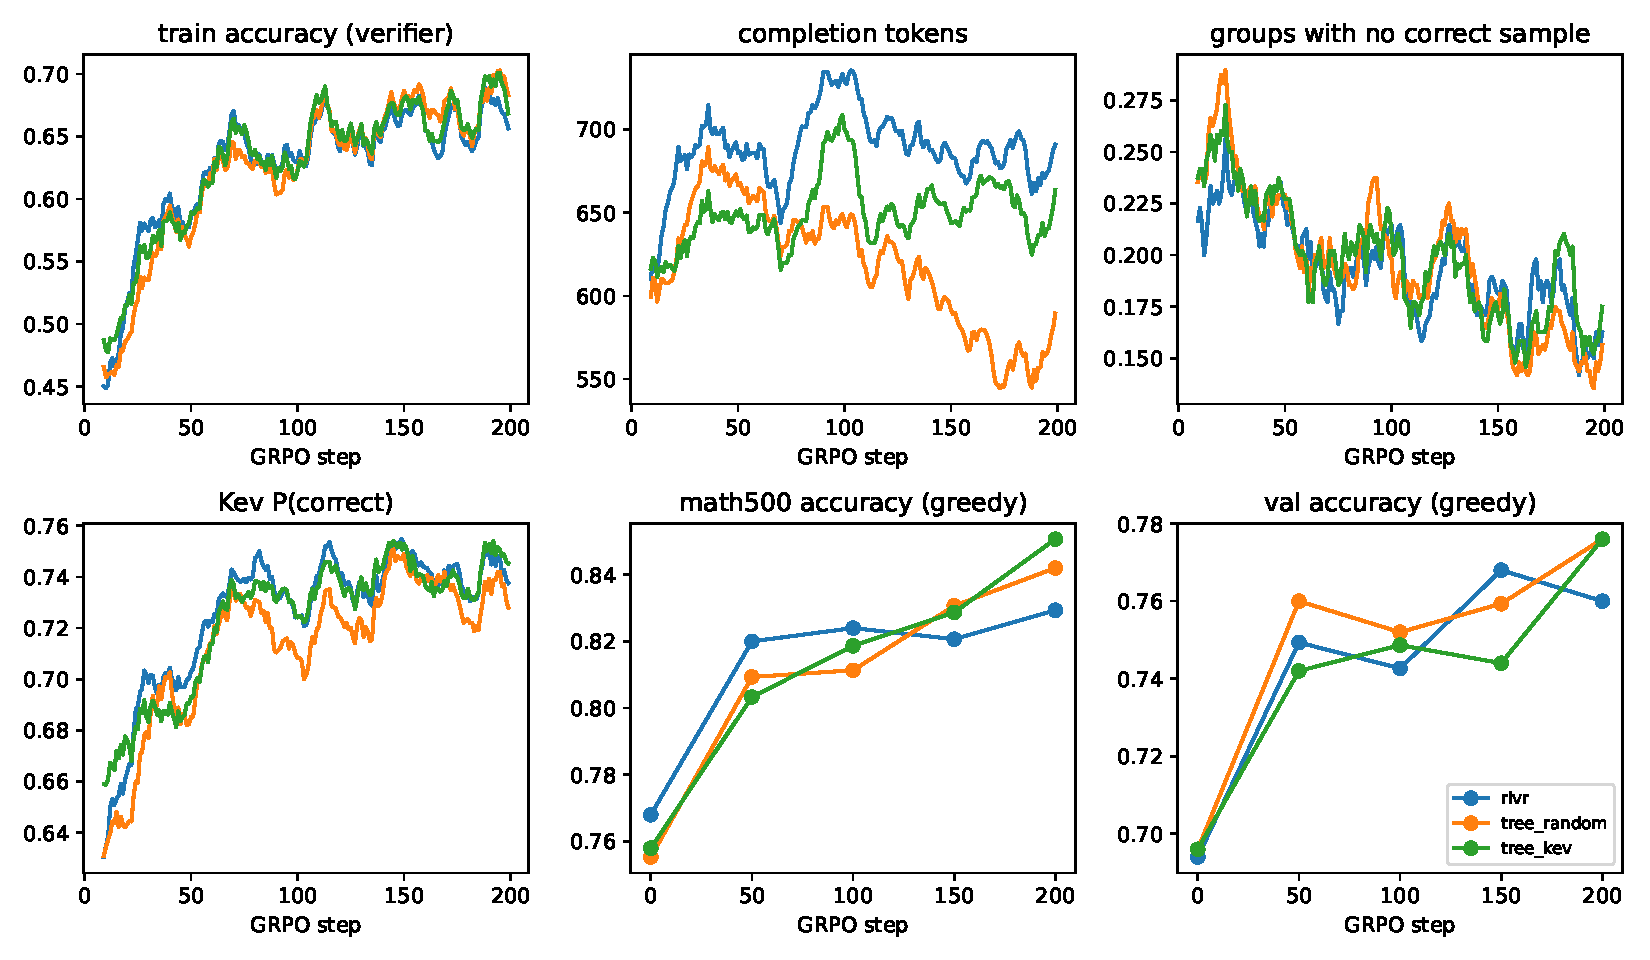
\includegraphics[width=\linewidth]{../../experiments/part3c_tree/results/training_curves.pdf}
\caption{Training curves (seed mean): verifier accuracy, completion tokens, share of groups with no correct completion
and \kev{}'s $\pc$ on the training completions (10-step moving averages), and greedy accuracy on MATH-500 and the
validation set every 50 steps.}
\label{fig:tree-curves}
\end{figure}

\paragraph{Evaluation noise.} Across the \NUM{szruns_math500} runs in this comparison, the base model's MATH-500
accuracy at step 0 ranges from \NUM{szmin_math500}\% to \NUM{szmax_math500}\%, and a run's accuracy changes by
\NUM{lecabs_math500} points on average between its evaluations at steps 150 and 200.

% Part III-C, discussion (included by main_en.tex).
% TODO when rlvr seed 3 is in: check the paragraph on the tree shape against its accuracies.

\section{Discussion}\label{sec:discussion}

\paragraph{Within a problem, the judge sees little of where a solution is going.} Offline, \kev{}'s \emph{on track}
score separates the correct from the incorrect continuations of one problem's 128-token prefixes with an AUROC of
\NUM{aucw_128_kevtrack}, no better than the AR judge of the same size (\NUM{aucw_128_artrack}) or the policy's own
log-probability (\NUM{aucw_128_logprob}), which costs nothing. Across problems every signal does better, because each
partly sees how hard the problem is, and that does not help to choose among one problem's prefixes. In training, on
the policy's own roots, the separation was weaker still (\NUM{auditotaucw_all_treekev}
\ci{\NUM{auditotaucwlo_all_treekev}}{\NUM{auditotaucwhi_all_treekev}}), and keeping \kev{}'s two roots of four raised
the share of correct leaves by \NUM{auditgain_all_treekev}
\ci{\NUM{auditgainlo_all_treekev}}{\NUM{auditgainhi_all_treekev}} points, against \NUM{auditgain_all_treerand} for a
random choice and \NUM{auditbest_all_treekev} for the best two in hindsight. The gain was larger early in training
(\NUM{auditgain_firsthalf_treekev} points in the first half, \NUM{auditgain_secondhalf_treekev} in the second, 20
audited steps each, without intervals), while the policy's roots came to lead to correct answers more often and the
room for a choice shrank (best two in hindsight: \NUM{auditbest_firsthalf_treekev} and
\NUM{auditbest_secondhalf_treekev} points).

\paragraph{A small gain at the roots did not change what the policy learned.} With the same tree shape, keeping
\kev{}'s roots instead of random ones left the final accuracy unchanged within the intervals over problems on four of
the five benchmarks; on GSM8K it was \NUM{dvtreerand_treekev_gsm}
\ci{\NUM{dvtreerandlo_treekev_gsm}}{\NUM{dvtreerandhi_treekev_gsm}} points higher, one interval of five over two seeds,
which we do not count as an effect. The idea behind the judge's choice is that it gives GRPO more groups with mixed
outcomes, the only groups with a learning signal. It did not: in the last 20 steps \NUM{allwrong_treekev} of the
groups had no correct leaf under \texttt{tree\_kev} and \NUM{allwrong_treerand} under \texttt{tree\_random}, and
\NUM{allright_treekev} and \NUM{allright_treerand} had only correct ones. The choice has a cost in principle: the kept
roots are no longer samples of the policy, so the gradient is no longer an unbiased estimate of the policy gradient.
We saw no effect of that on accuracy. One seed of \texttt{tree\_kev} came to repeat its solution after the first
answer, which neither seed of \texttt{tree\_random} did. Its reward is the verifier's alone, which does not penalise a
repetition that restates the answer, so this is not the judge paying for repetition; whether the choice of roots
caused it, one seed of two cannot tell.

\paragraph{Whether the tree shape helps is open.} Both tree conditions end above flat sampling in the seed mean, by
\NUM{d_treerand_math} and \NUM{d_treekev_math} points on MATH-500 and \NUM{d_treerand_aime24} and
\NUM{d_treekev_aime24} on AIME24, and \texttt{tree\_random} generated fewer tokens per step than flat sampling
(\NUM{gentok_treerand} thousand against \NUM{gentok_rlvr} thousand). But each tree condition has one seed well above
\texttt{rlvr} and one at its level, and at step 100 neither was ahead. The intervals over problems do not include the
variation between seeds, and with two seeds per condition the difference may be the seeds'. Testing the tree shape
needs more seeds than we ran.

\paragraph{Limitations.} One policy size (4B), one judge question (\emph{on track}) asked of 128-token roots, one tree
shape (four roots, two kept, four leaves each), 200 steps at the learning rate of Part II, and \NUM{seeds_treekev}
seeds per tree condition (\texttt{rlvr}: \NUM{seeds_rlvr}). With more roots per prompt a judge has more to choose from,
and so do its errors. The audit continues all roots only every tenth step, 20 audited steps per run; its intervals
resample those steps, not seeds. The offline study used the base policy's prefixes, not the training policy's. We
report tokens, not time: the runs shared GPUs with other experiments.

\paragraph{Relation to the earlier versions.} Versions 1--3 of this paper reported pruning speed-ups, KV-cache reuse
rates, per-node latencies and theorem-proving results (MiniF2F-Lean4, ProofNet) that were not measured (see the notice
at the start and \file{CORRECTION.md}). None of these is measured here: we count tokens, not time, and ran no theorem
proving. What we could test, we did. The pruning rule of v3, prune a prefix when the judge's $p(\text{yes})<0.3$,
prunes \NUM{thrpruned_128_kevtrack} of the 128-token prefixes with the \emph{on track} question and catches
\NUM{thrcaught_128_kevtrack} of the dead ones (\S\ref{sec:res-prefix}). Choosing which roots to continue by \kev{}, the
idea behind those versions, did not make GRPO learn better than a random choice of roots.


\section*{Reproducibility}
Code, prompts, raw logs (every GRPO step and evaluation) and the prefix study's solutions, prefixes, continuations and
judge scores are in the repository (\file{experiments/part3c_tree/}). The tables and every number in the text are
generated from them by \file{dcjev/llm/prefix_study.py}, \file{dcjev/analysis/part2.py} and
\file{dcjev/analysis/paper_numbers.py}.

\bibliographystyle{plainnat}
\bibliography{../common/refs}
\end{document}
